\section{Introduction}
\label{sec:eval_intro}
In this chapter, detail setting, result, and analysis of our experiments are discussed.
Section~\ref{sec:eval_setdetail} details hardware configurations and data set we use. 
There are 5 experiments conducted. In Section~\ref{sec:eval_diffval}, we discuss the experiment 
where we assess runtime to access object's field with different variable types. 
Section~\ref{sec:eval_refcount} shows details to examine how behaviors of normal reference and Reference Count are different. 
Section~\ref{sec:eval_sort} describes our Merge-sort experiment to examine behavior of Atomic Reference Counting.
Two algorithms are discussed used in Big Data processing and examined in our experiments: 
Tree-aggregate in Section~\ref{sec:concept_treeagg} and K-Nearest-Neighbors in Section~\ref{sec:concept_knn}.

\section{Experimental Set and Detail}
\label{sec:eval_setdetail}
\subsection{Wikipedia Data Sets}
 \label{sec:concept_dataset}
 Wikipedia page data sets are used to perform document classification with KNN. 
 \(10^5\) pages are used for training data set, and 18724 pages are used for target.

 \subsection{Experimental Details}
 \label{sec:concept_expdetail}
 Our experiments are run on three types of VM instances on Google Cloud Platform: 
 n1-standard-1 which has 1 vCPU, 3.75 GB RAM, and 10 GB Standard persistent disk, 
 n1-standard-4 which has 4 vCPU, 15 GB RAM, and 10 GB Standard persistent disk, 
 n1-standard-8 which has 8 vCPU, 30 GB RAM, and 10 GB Standard persistent disk,  
 All of the experiments described are performed 5 times. 
 In this thesis, we present the average of 5 separate runs for each experiment.

\section{Experiment 1: Accessing Object with Different Variable Type}
\label{sec:eval_diffval}
This experiment is conducted to provide answers to the following two questions. One is how different variable types have impact to runtime performance.
The other is how initialization of Vec size has impact to runtime performance. 
In this experiment, we focus on owner, reference, and slice as a variable of sequence values. 
Since these variables have different memory representation, there might be differences among time for access to actual values of each variables.

To evaluate this assumption, we use the three types of complex object: CustomerOwned, CustomerBorrowed and CustomerSlice. 
At first, we generate source Vecs for all fields, Vecs which contain all elements used for corresponding fields of objects.
For example, all of i32 elements used for key field in 1 million Customer object are stored in Vec$<$i32$>$ with 1 million i32 elements. 
Later, these i32 elements are moved to be owned or borrowed by the object's fields.

Next, 3, 13, 23, 33 million of Customer objects are created and stored in Vec. 
When a Customer Vec is created, whether size of Vec is initialized is controlled. 
Finally, serialization of Customer object is performed as an operation forcing program to access all of fields in the object.
This serialization is performed each Customer objects in the Vec. We measure total runtime to serialize all of Customer objects 
stored in Vec. 

\subsection{Result}
\label{sec:history}
The result is shown in Figure~\ref{fig:rustaccessinit} and Figure~\ref{fig:rustaccessnoinit}.
Figure~\ref{fig:rustaccessinit} is comparison of the runtime performance among different Customer object types with Vec size initialization.
Figure~\ref{fig:rustaccessnoinit} is comparison in the same set of experiment except Vec size is not initialized. 
The blue, yellow, and green chats represent runtime of access to fields of CustomerOwned, CustomerBorrowed, and CustomerSlice objects respectively.

No matter Vec size initialized or not, differences of runtime for accessing objects are not remarkable among different object types. 


\begin{figure}[htb]
    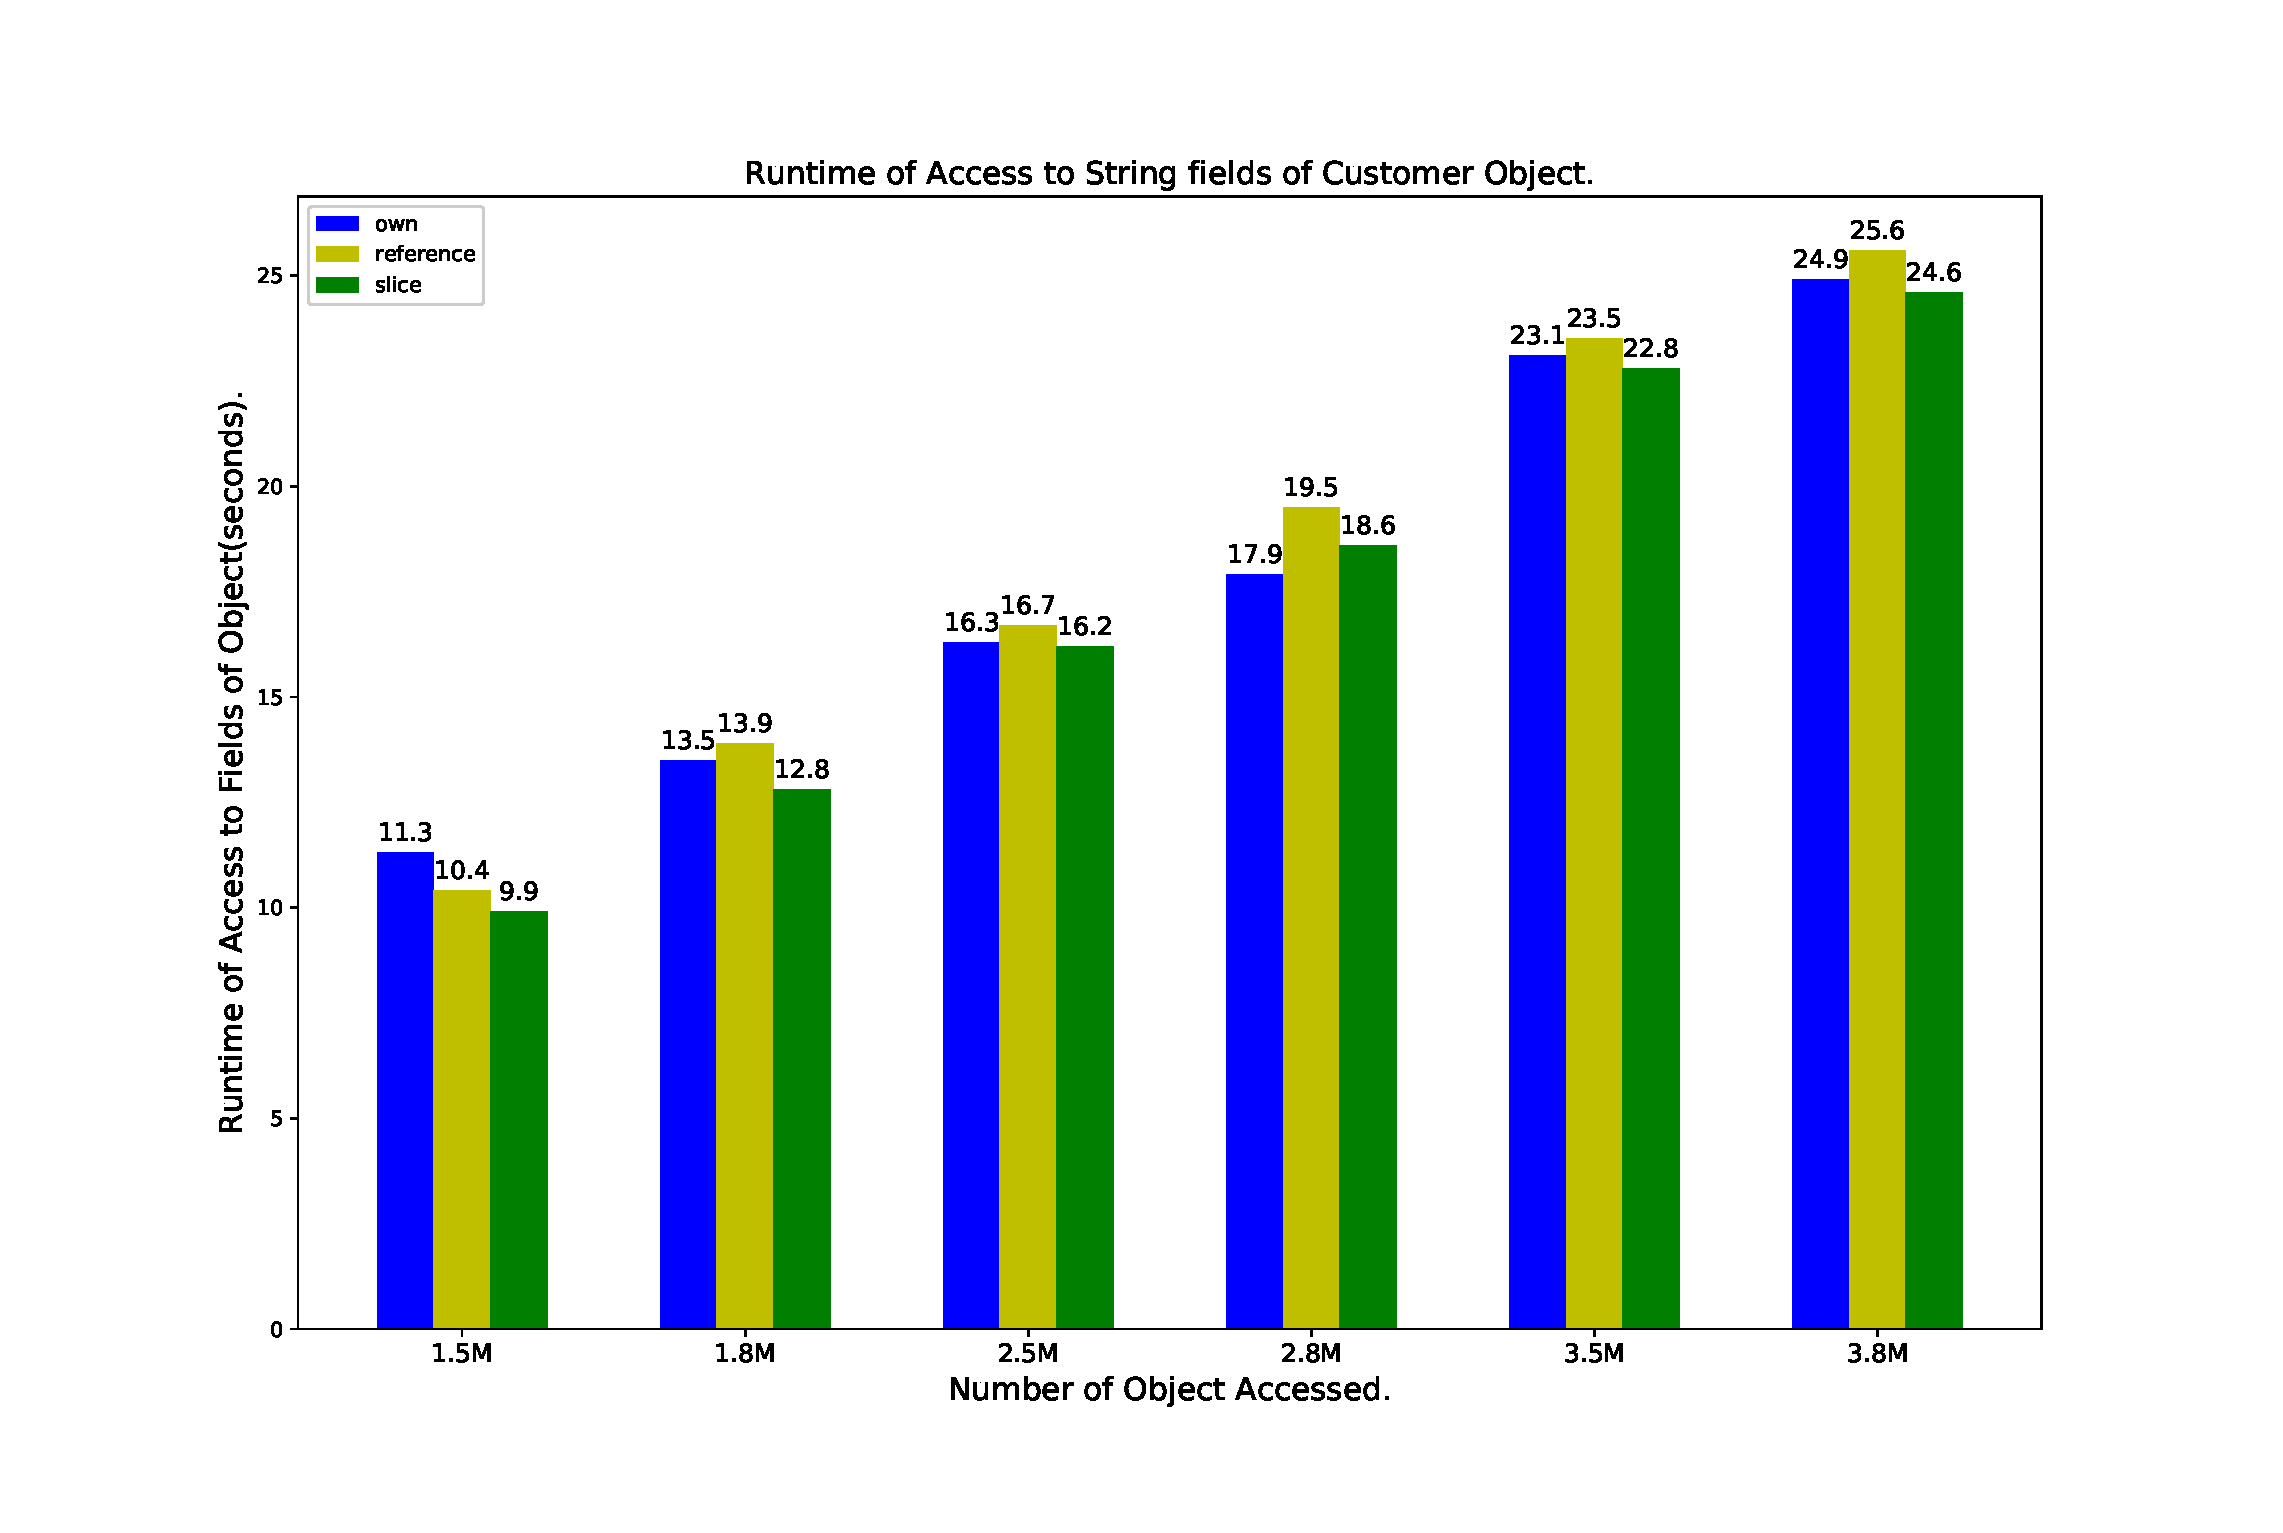
\includegraphics[width=15cm]{rust_access_different_poniter_init.eps}
    \caption{Runtime of Access to Different Pointer Types with Vec Size Initialization}
    \label{fig:rustaccessinit}
\end{figure}

\begin{figure}[htb]
    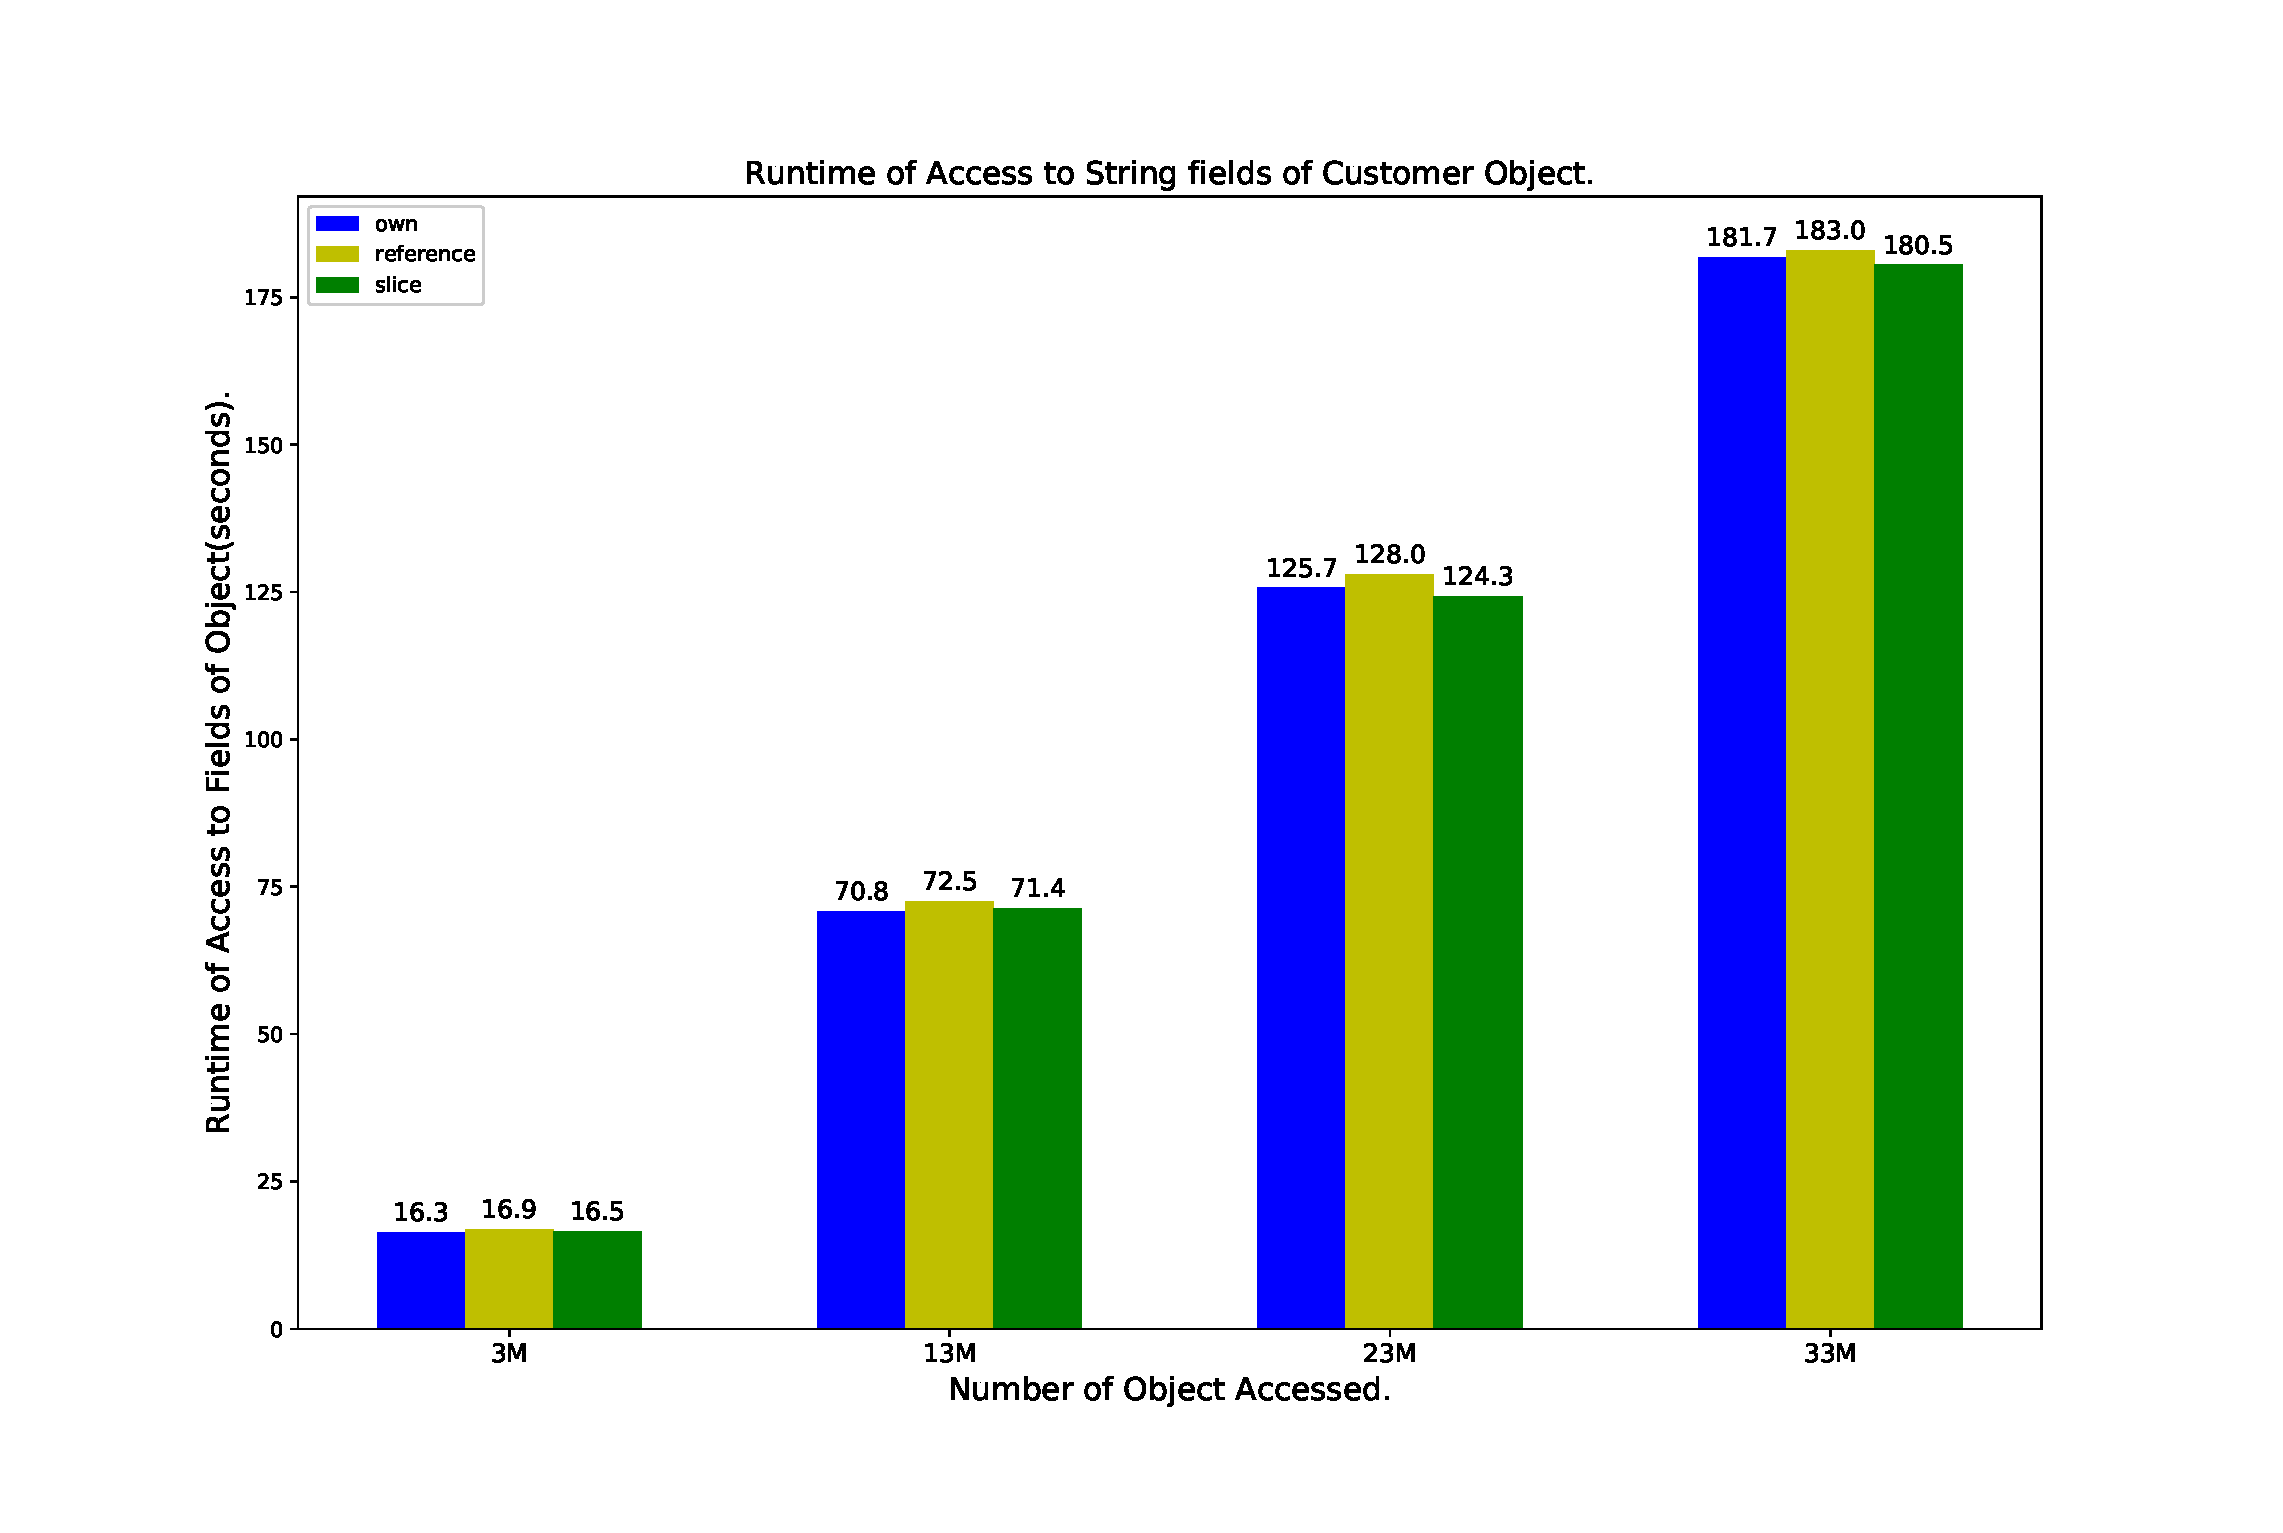
\includegraphics[width=15cm]{rust_access_different_poniter_noinit.eps}
    \caption{Runtime of Access to Different Pointer Types without Vec Size Initialization}
    \label{fig:rustaccessnoinit}
\end{figure}


% \begin{figure}[htb]
%     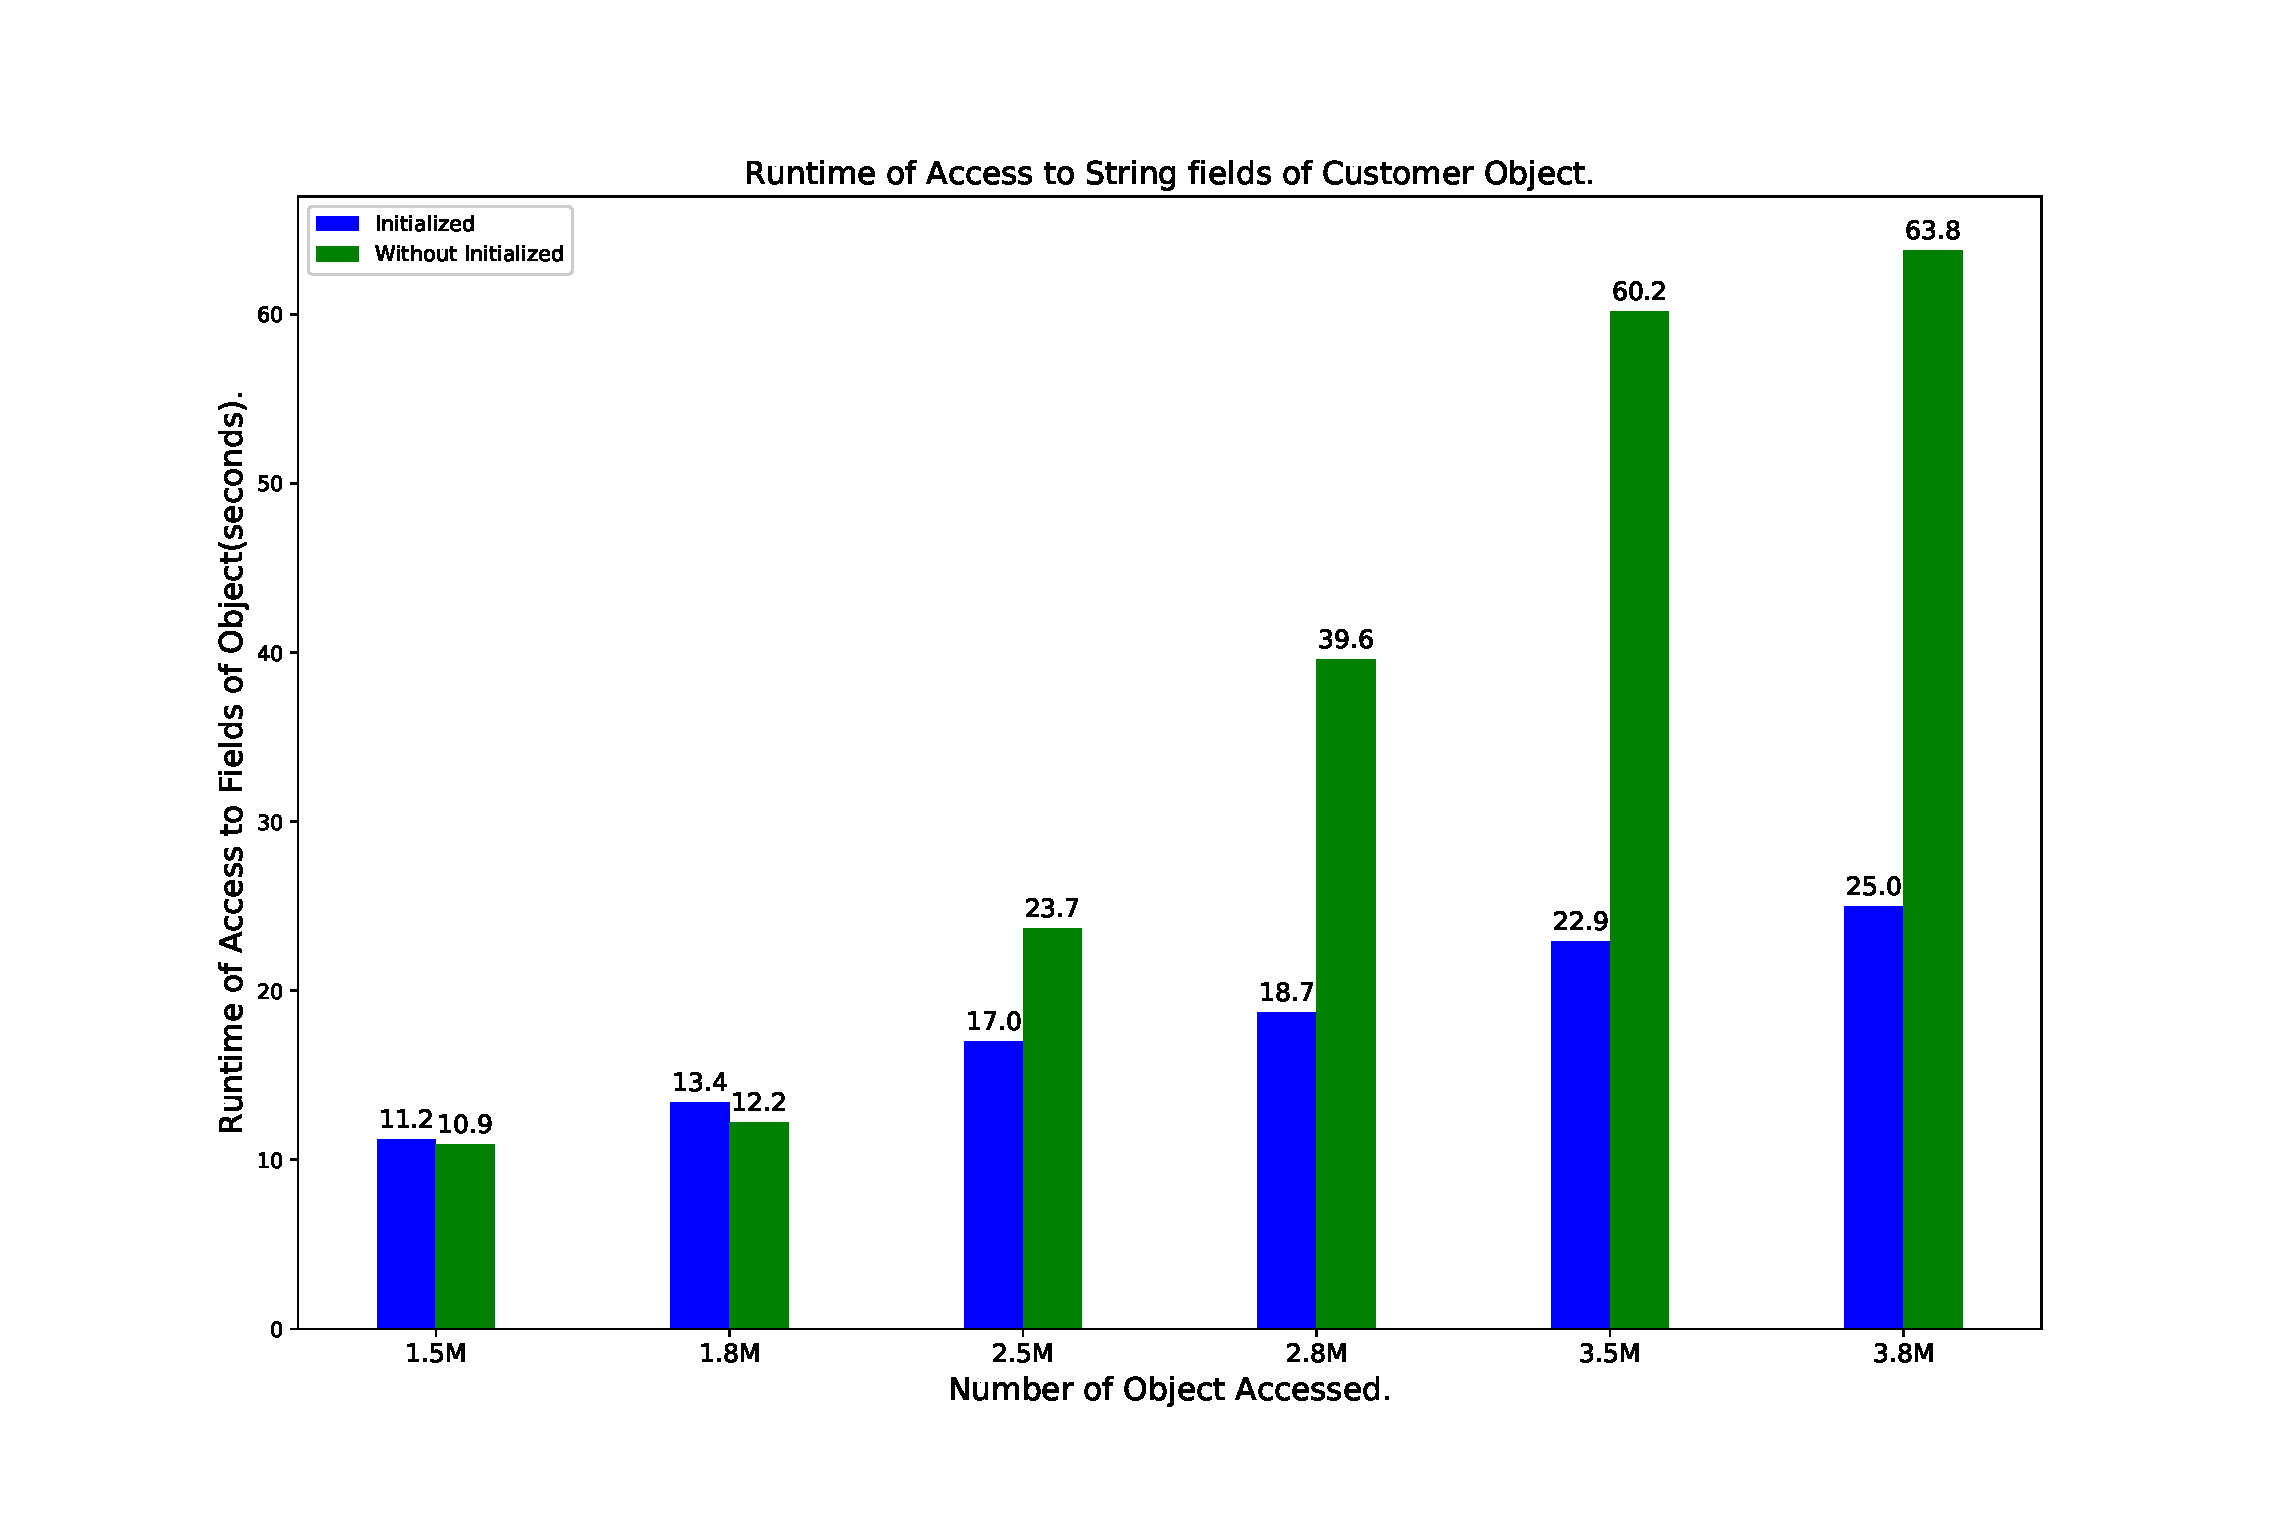
\includegraphics[width=15cm]{rust_access_init_vs_noint.eps}
%     \caption{Runtime of Access to Fields of Complex Object with Initialization vs without Initialization}
%     \label{fig:init_vs_noinit}
% \end{figure}

\subsection{Discussion}
\label{sec:history}
Difference of variable types does not have huge impact to runtime of accessing to actual value.
Even thought owner, reference , and slice have different memory representations, the access time to its value is 
close to each other. As shown in Figure~\ref{fig:own_ref_slice}, the representations of owner and slice are almost identical except slice does not have capacity for values.
Reference is pointer pointing to owner, so it has an additional step to access actual value. 
However, the result shows this additional step does not have huge impact for runtime to access memory region of the value.

% Whether initializing Vec size results in disparity of runtime performance to access objects' fields. 
% This is because when Vec uninitialized, the elements of Vec are allocated across different virtual memory pages.



\section{Experiment 2: Assessment of different reference methods in Rust}
\label{sec:eval_refcount}
% In Rust programming, a reference is a pointer to reduce unnecessary movement of ownership. 
% One use case is where we pass reference to values to arguments of function. 
% If we pass owner to function, the owner is moved and the corresponding value is deallocated when the call of function ends. 
% To avoid this, the owner should always be returned. This may be an encumbrance while complex software system development. 
% By using reference, we do not have to worry about returning it, because reference is an additional pointer to an owned value. 
% Reference can be used for operation in the same way of owner, but also be moved without deallocation of value by keeping its owner live. 

% Reference is useful to avoid movement of ownership. However, one needs to track its lifetime and explicitly includes it in code, 
% because Rust compiler cannot infer it. This can be another encumbrance. We can instead acquire multiple owners to single value by using Reference Counting (Rc). 
% By leveraging Rc, a value can be shared like what borrowing plays the role in Rust programming. 
% The difference is that Rc checks number of owner pointing to the actual data and makes sure the data is not deleted 
% until all the owners are dereferenced. Using Rc is sometimes preferable approach for developers especially when lifetime planning is extremely difficult.
% However, the possible problem regarding to Rc is the cost for tracking the number of references. 
% Having this assumption, this experiment will show difference of behavior among Rc and simple reference.

In this experiment, CustomerBorrowed and CustomerRc are used to see difference of dropping time among reference and Rc. 
In the CustomerRc and OrderRc struct, all fields take Rc (Rc$<$T$>$). Similarly to the experiment in the last section, 
sets of integer, float, and String vector are created and their elements are borrowed or reference counted to create CustomerBorrowed or CustomerRc objects.
The dropping of objects deletes references or Rcs used for fields of the objects. However, it does not deallocate values to which they are pointing. 
Therefore, the evaluated runtime of dropping objects only consists of dropping time of reference or Rc, but deallocation time.
We generated 10, 20, 30, and 40 million CustomerBorrowed and CustomerRc objects and performed drop one by one. 

\subsection{Result}
Figure\ref{fig:rc_ref} shows comparison of runtime dropping CustomerBorrowed and CustomerRc objects. 
The result shows significant difference of dropping time among the two objects; deletion of CustomerRc is much slower than CustomerBorrowed. 
The runtime of dropping CustomerBorrowed is about 60 times faster than dropping CustomerRc. 
The memory usage for algorithms with 40 million of Customer objects are about 26G bytes for both CustomerRc and CustomerBorrowed.

\begin{figure}[htb!]
    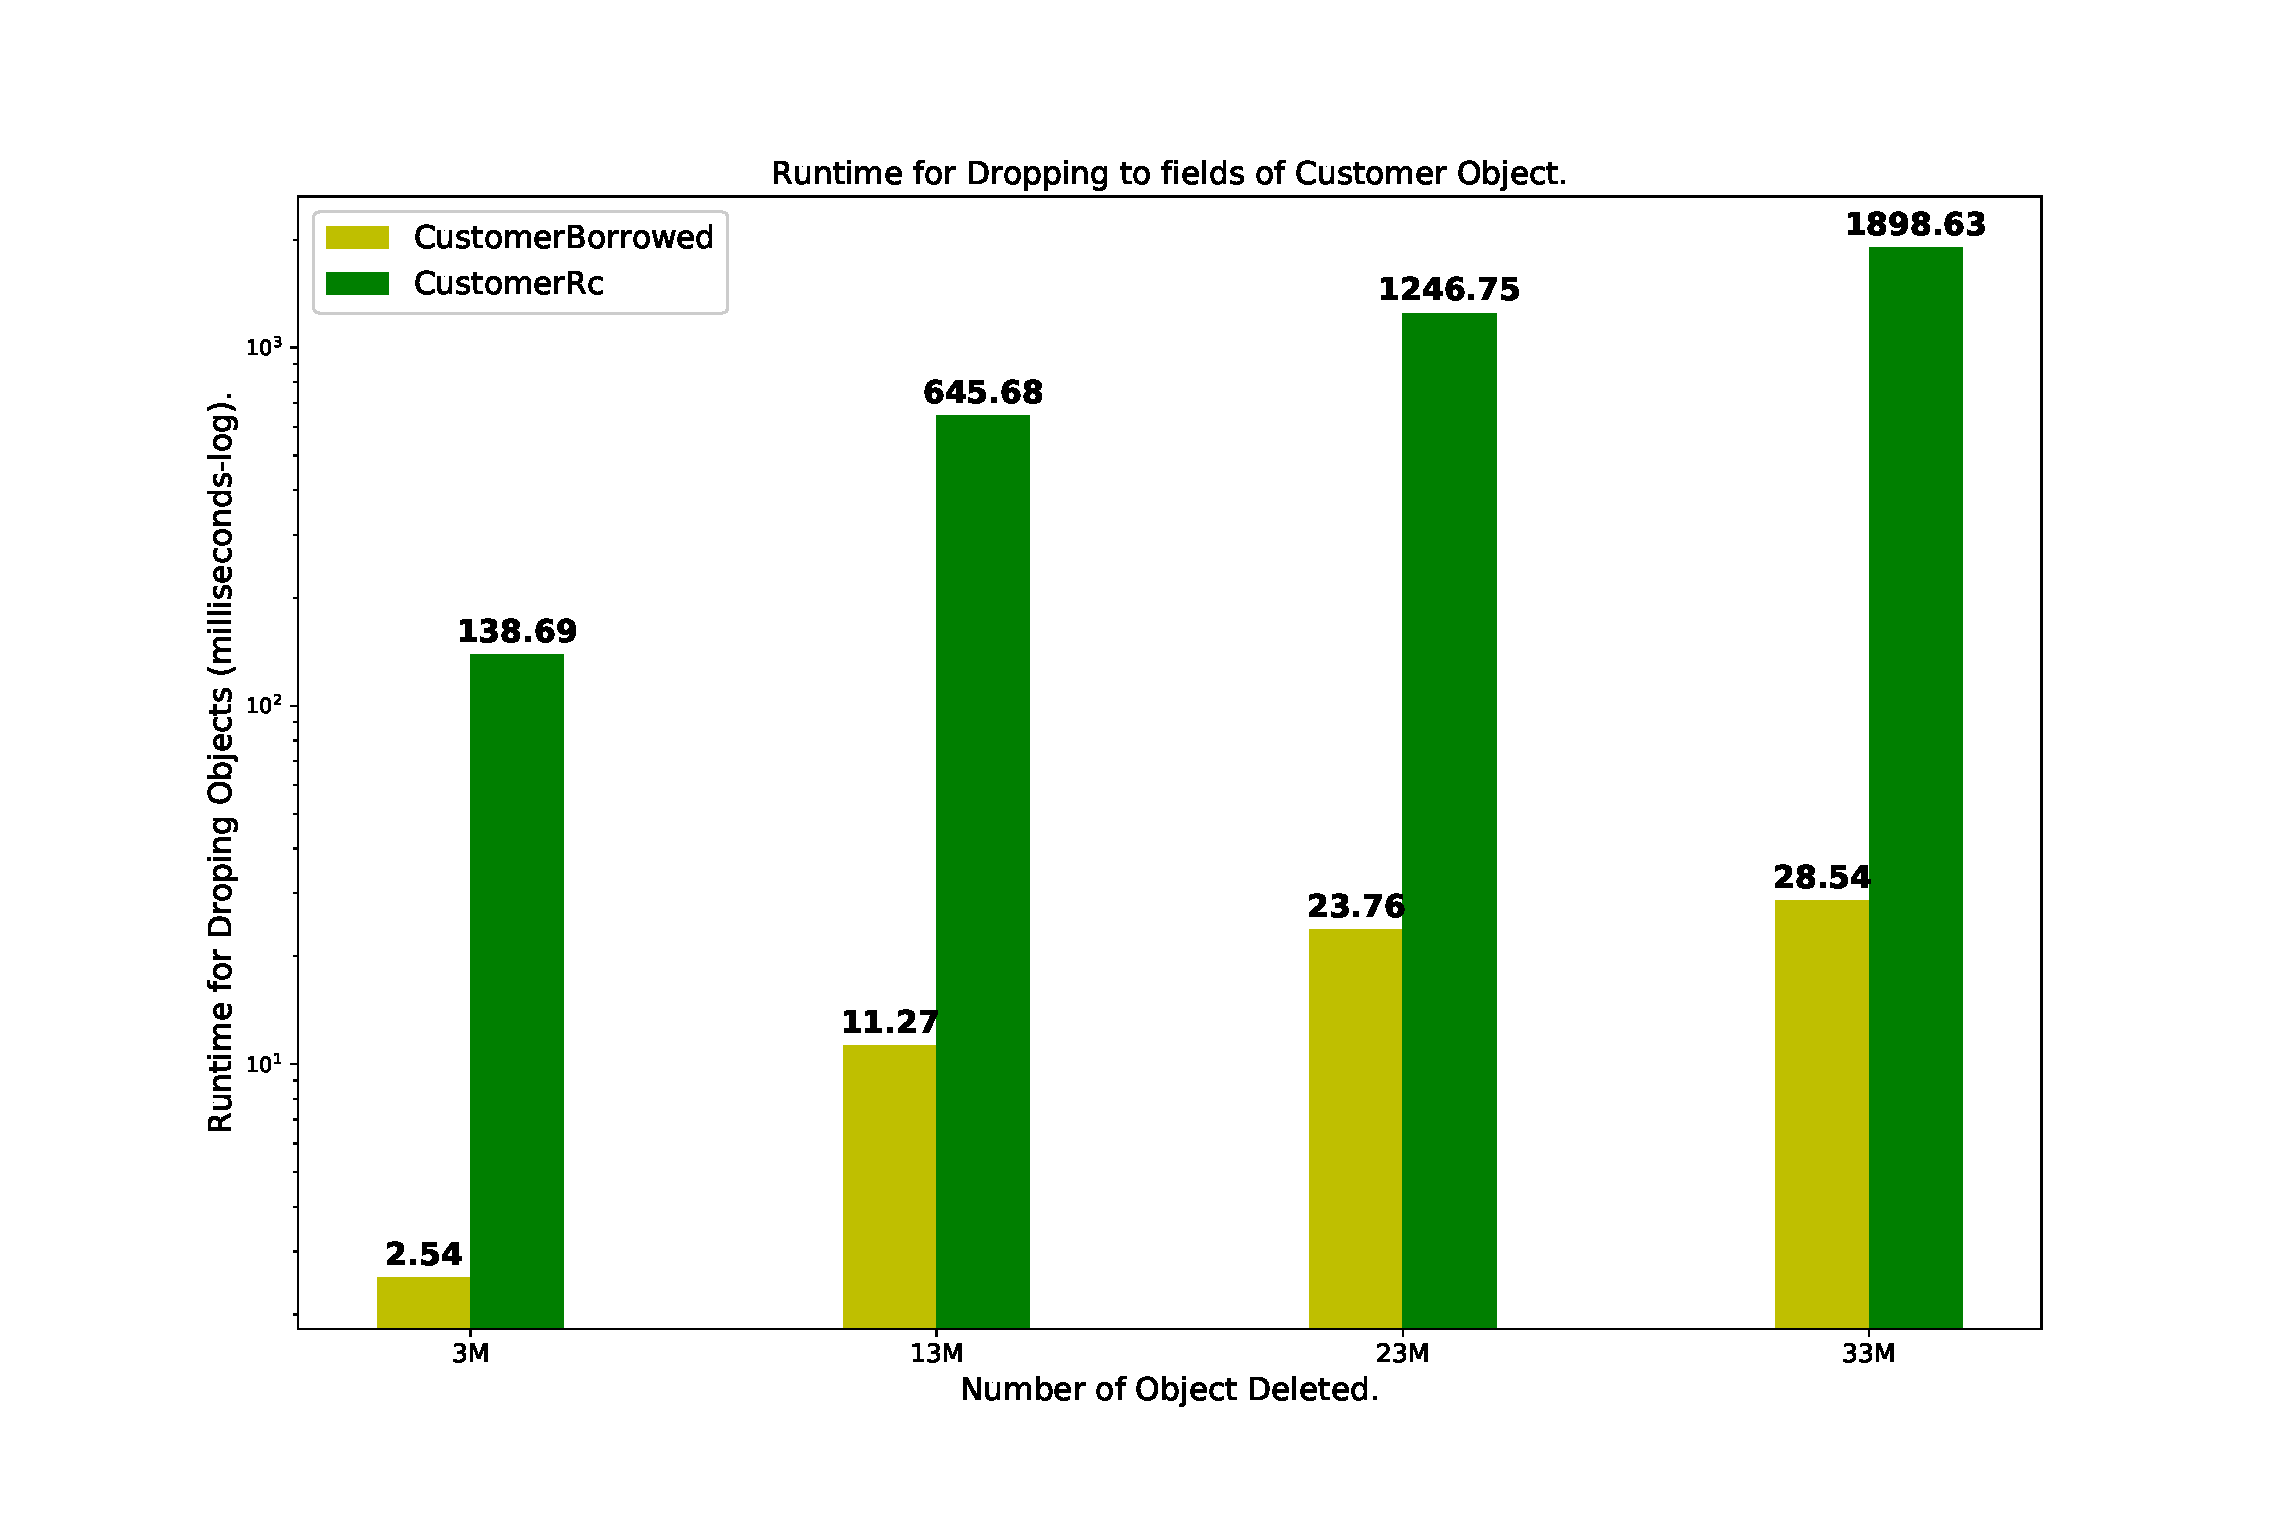
\includegraphics[width=15cm]{rust_droptime_borring_rc.eps}
    \caption{Runtime for dropping Customer Object}
    \label{fig:rc_ref}
\end{figure}


\subsection{Discussion}
In this experiment, an assessment is conducted to verify whether there is difference between behavior of reference and Rc.
The reason why dropping Rc is much slower than dropping reference is that Rc requires runtime overhead to check some states of the variable, 
but when to drop reference is already determined at compile time. When dropping Rc, Rc has to check the number of variables pointing to the actual content and decide 
whether to deallocate the memory or not. However, memory management and lifetime strategy of reference is already determined at compile time.
This determination of memory management strategy at compile increases runtime performance of dropping complex object constructed with reference type variable.
This may say that we should use reference whenever high performance computation is critical.

However, dealing with reference is sometimes cumbersome. Tracking lifetime of reference can be done easily in simple situation. 
But, if we have complex objects constructed with fields of reference, the lifetime tracking becomes extremely difficult. 
For example, constructing nested objects with reference fields requires a developer to plan memory management with many lifetime symbols. 
Using reference counting eliminates the developer's responsibility to specify lifetime of variables. 
This may ease and speed up development process, and increase understandability of codes.

Even though we have stack allocated values, such as i32 and f64, in Rc in our experiment, 
one should avoid wrapping stack allocated values in Rc. Wrapping value in Rc allocates heap memory so that allocating Rc$<$i32$>$ or Rc$<$f64$>$ unnecessarily uses space of 
heap. Additionally, stack allocated values are usually easy to be copied. Therefore, developer does not have to even use reference; one can just copy the value. 
Copying value in Rust is to copy the original value and to assign the copy to new owner variable. 

\section{Experiment 2: Merge-sort}
\label{sec:eval_sort}
This experiment is to assess importance of careful memory management in multithreading of Rust. 
We implement merge-sort algorithm in two different ways. One is sharing source vector with Arc. 
The other is passing slice of source vector to child thread. 

Our merge-sort algorithm with vector is implemented with recursion. In these alogorithm, the splitting phase is merely aquiring index of split position, 
not actually splitting the source vector. At merge phase, merge function receives two independent vector and merge these into single new vector.

For sharing data implementaion, channel with sending data is used for multithreading method, because we want to ensure children threads return values before parent thread proceed execution. 
For passing slice implementation, we use scope method to enable children threads to receive reference from their parent ensuring the same purpose of sending data. 

Experiment performed is the comparison among sharing data and passing slice implementations to see the impact of Arc, Atomic reference conuting, to runtime performance.
These two implementations are theoritically the same operations other than using or not using Arc to share data. 
This comparison can effectively show how important careful memory management is in multithreading computation in Rust. 
In another word, how atomic reference counting can cost for computation in Rust programming.

The figure shows the result of 
An atomic reference count of the shareable vector is passed to every recursion steps and 


\begin{figure}[htb]
    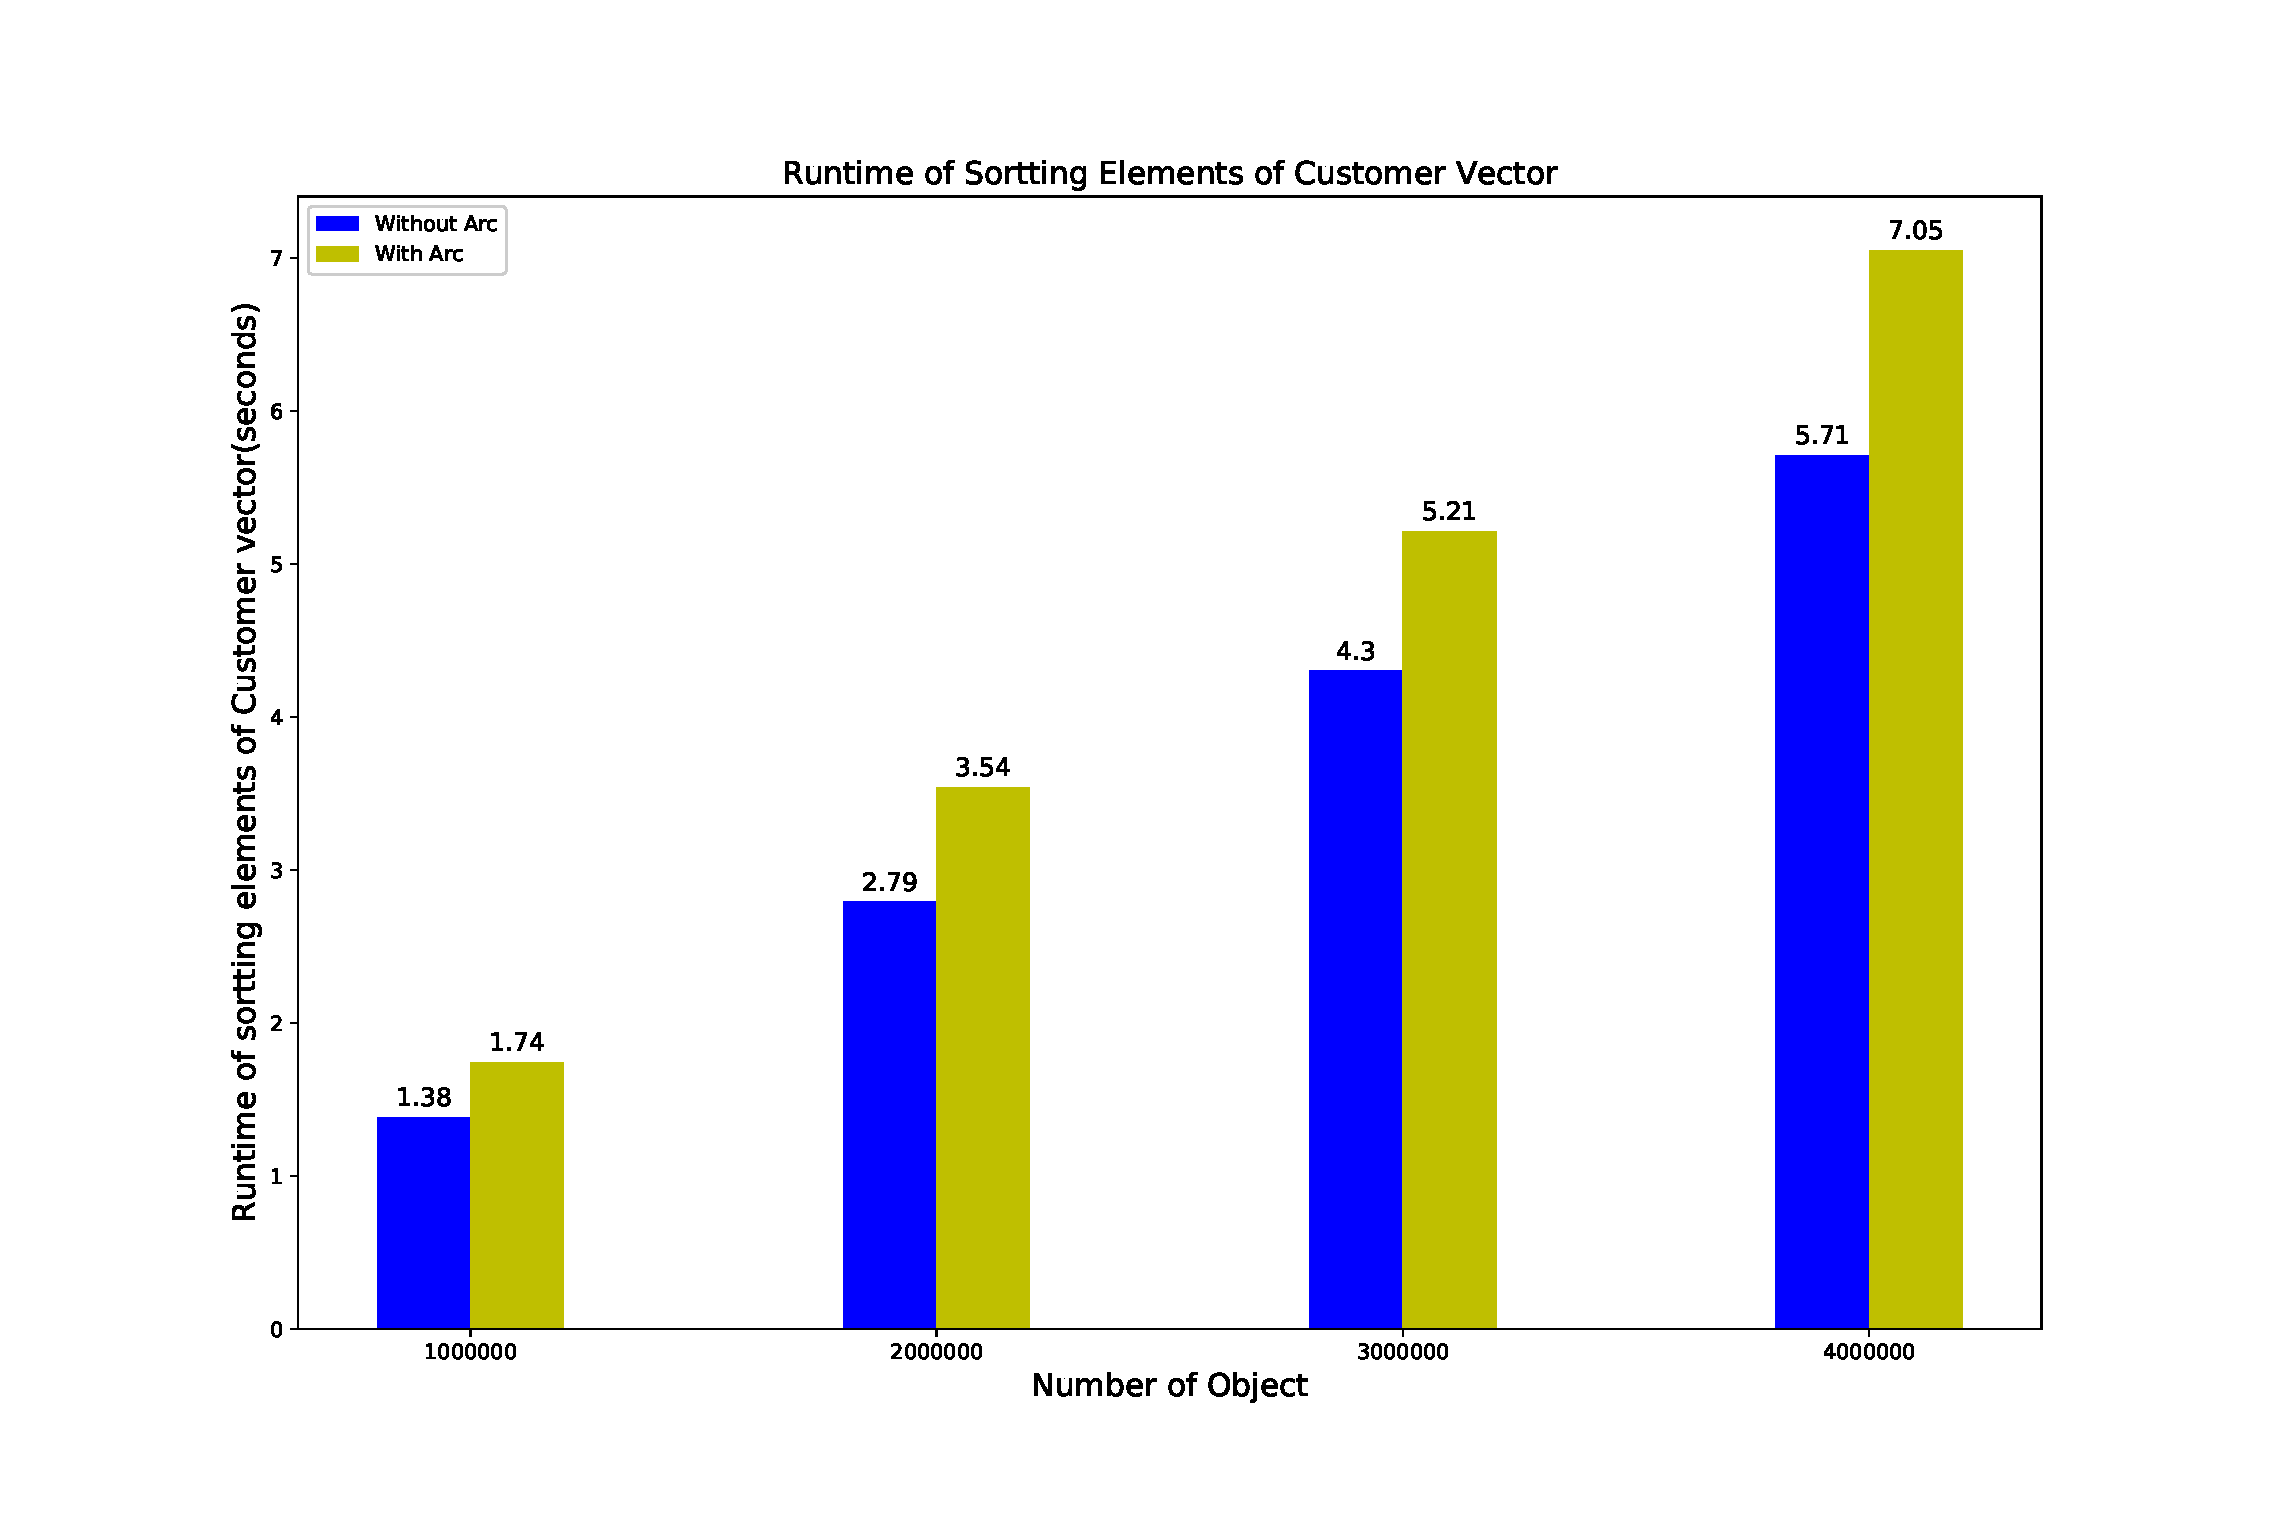
\includegraphics[width=15cm]{rust_merge_sort.eps}
    \caption{Runtime of Sortting Elements of Customer Vector}
    \label{fig:Sampling}
\end{figure}



The other is LinkedList implementation other than vector.
The linkedlist implementation is different from another two. This algorithm is inplace sorting so that it does not de/allocate memory during execution. 
The comparison among vector and linkedlist implementations can show trade-off between contiguous memory access and inplace non memory de/allocation. 
Experiment with Java linkedlist implementation can be interesting, because Java GC is severe problem when number of object is large. 


\section{Experiment 4: Tree-aggregation}
\label{sec:eval_treeagg}
\subsection{Description}
Tree-aggregate is a communication patten heavily used for Machine Learning algorithm in Spark (MLlib). 
In the traditional aggregation function in Spark, results of aggregation in all executor clusters are sent to the driver. 
That is why this operation suffers from the CPU cost in merging partial results and the network bandwidth limit.
Tree-aggregate is a communication pattern which overcomes these problems by breaking aggregate operation in multi-level represented like tree structure.

In our experiment, tree-aggregation algorithms are examined in multi-threading. This experiment is to evaluate the impact of having Arc (Atomic Reference Counting) as elements of vector. 
In Big Data mining tool, such as Spark, it generates intermediate objects from original source vector. In tree-aggregation, aggregated HashMap like data structure is created in each step or node. 
Acquisition of elements in source vector is required to perform this aggregation. There are several ways.

One way is deep-copy elements of vector. This solution allocated newly created objects by deep-copy. 
Aggregation is performed on copied objects, stores them in the data structure and sends it to next node. 
Deep-copy generates duplicates of objects in vector and aggregated data structure. 
This can lead to memory intensive moment when we need memory space for the duplicated objects in addition.

The other way is to get reference to the elements. Since an original source vector is deallocated after a local aggregation,
Simple reference to elements does not live long enough and allow the aggregation result to be sent to next node. 
Instead of simple borrowing, we need owner in the aggregation result. Reference Counting (Rc) in Rust is a way to have multiple owners to a value. 
Since our experiment is implemented in multithreading, Atomic Reference Counting (Arc) is used instead of Rc. With Arc, multiple ownership pointer can be 
possessed by different variables across multiple threads. Therefore a value is not deallocated until all of owners to it are dropped. 
This does not require extra memory allocation, because only acquisition of new ownership to value is needed. 
However, deletion of Arc type checks whether the value is still owned by other variables. 
This checking may be a overhead in algorithms where generate a lot of intermediate data structures, because deletion of the data structures occurs in frequent.

Two algorithms are implemented using the above two different methods and evaluated their runtime performance. 
The both algorithms perform tree-aggregation where runs seven nodes. 
Each node load Customer vector from disk and aggregate it by Customer last name. Once a node finishes aggregation, it sends result to parent node. 
After parent nodes receive aggregation results from all of its children nodes, it joins all aggregation results including its and sends next parent. 
One algorithm performs aggregation by deep-copying elements from source vector loaded from disk. In the other algorithm, each element of source vector 
is wrapped in Arc, and its reference is acquired while aggregation. 


\subsection{Result}

Figure shows runtime performance of two tree-aggregate algorithms. The runtime of algorithm with deep-copy is slower than algorithm with Arc for every vector size. 
This is result of overhead of deep-copy is larger than deletion of Arc. 

\begin{figure}[htb]
    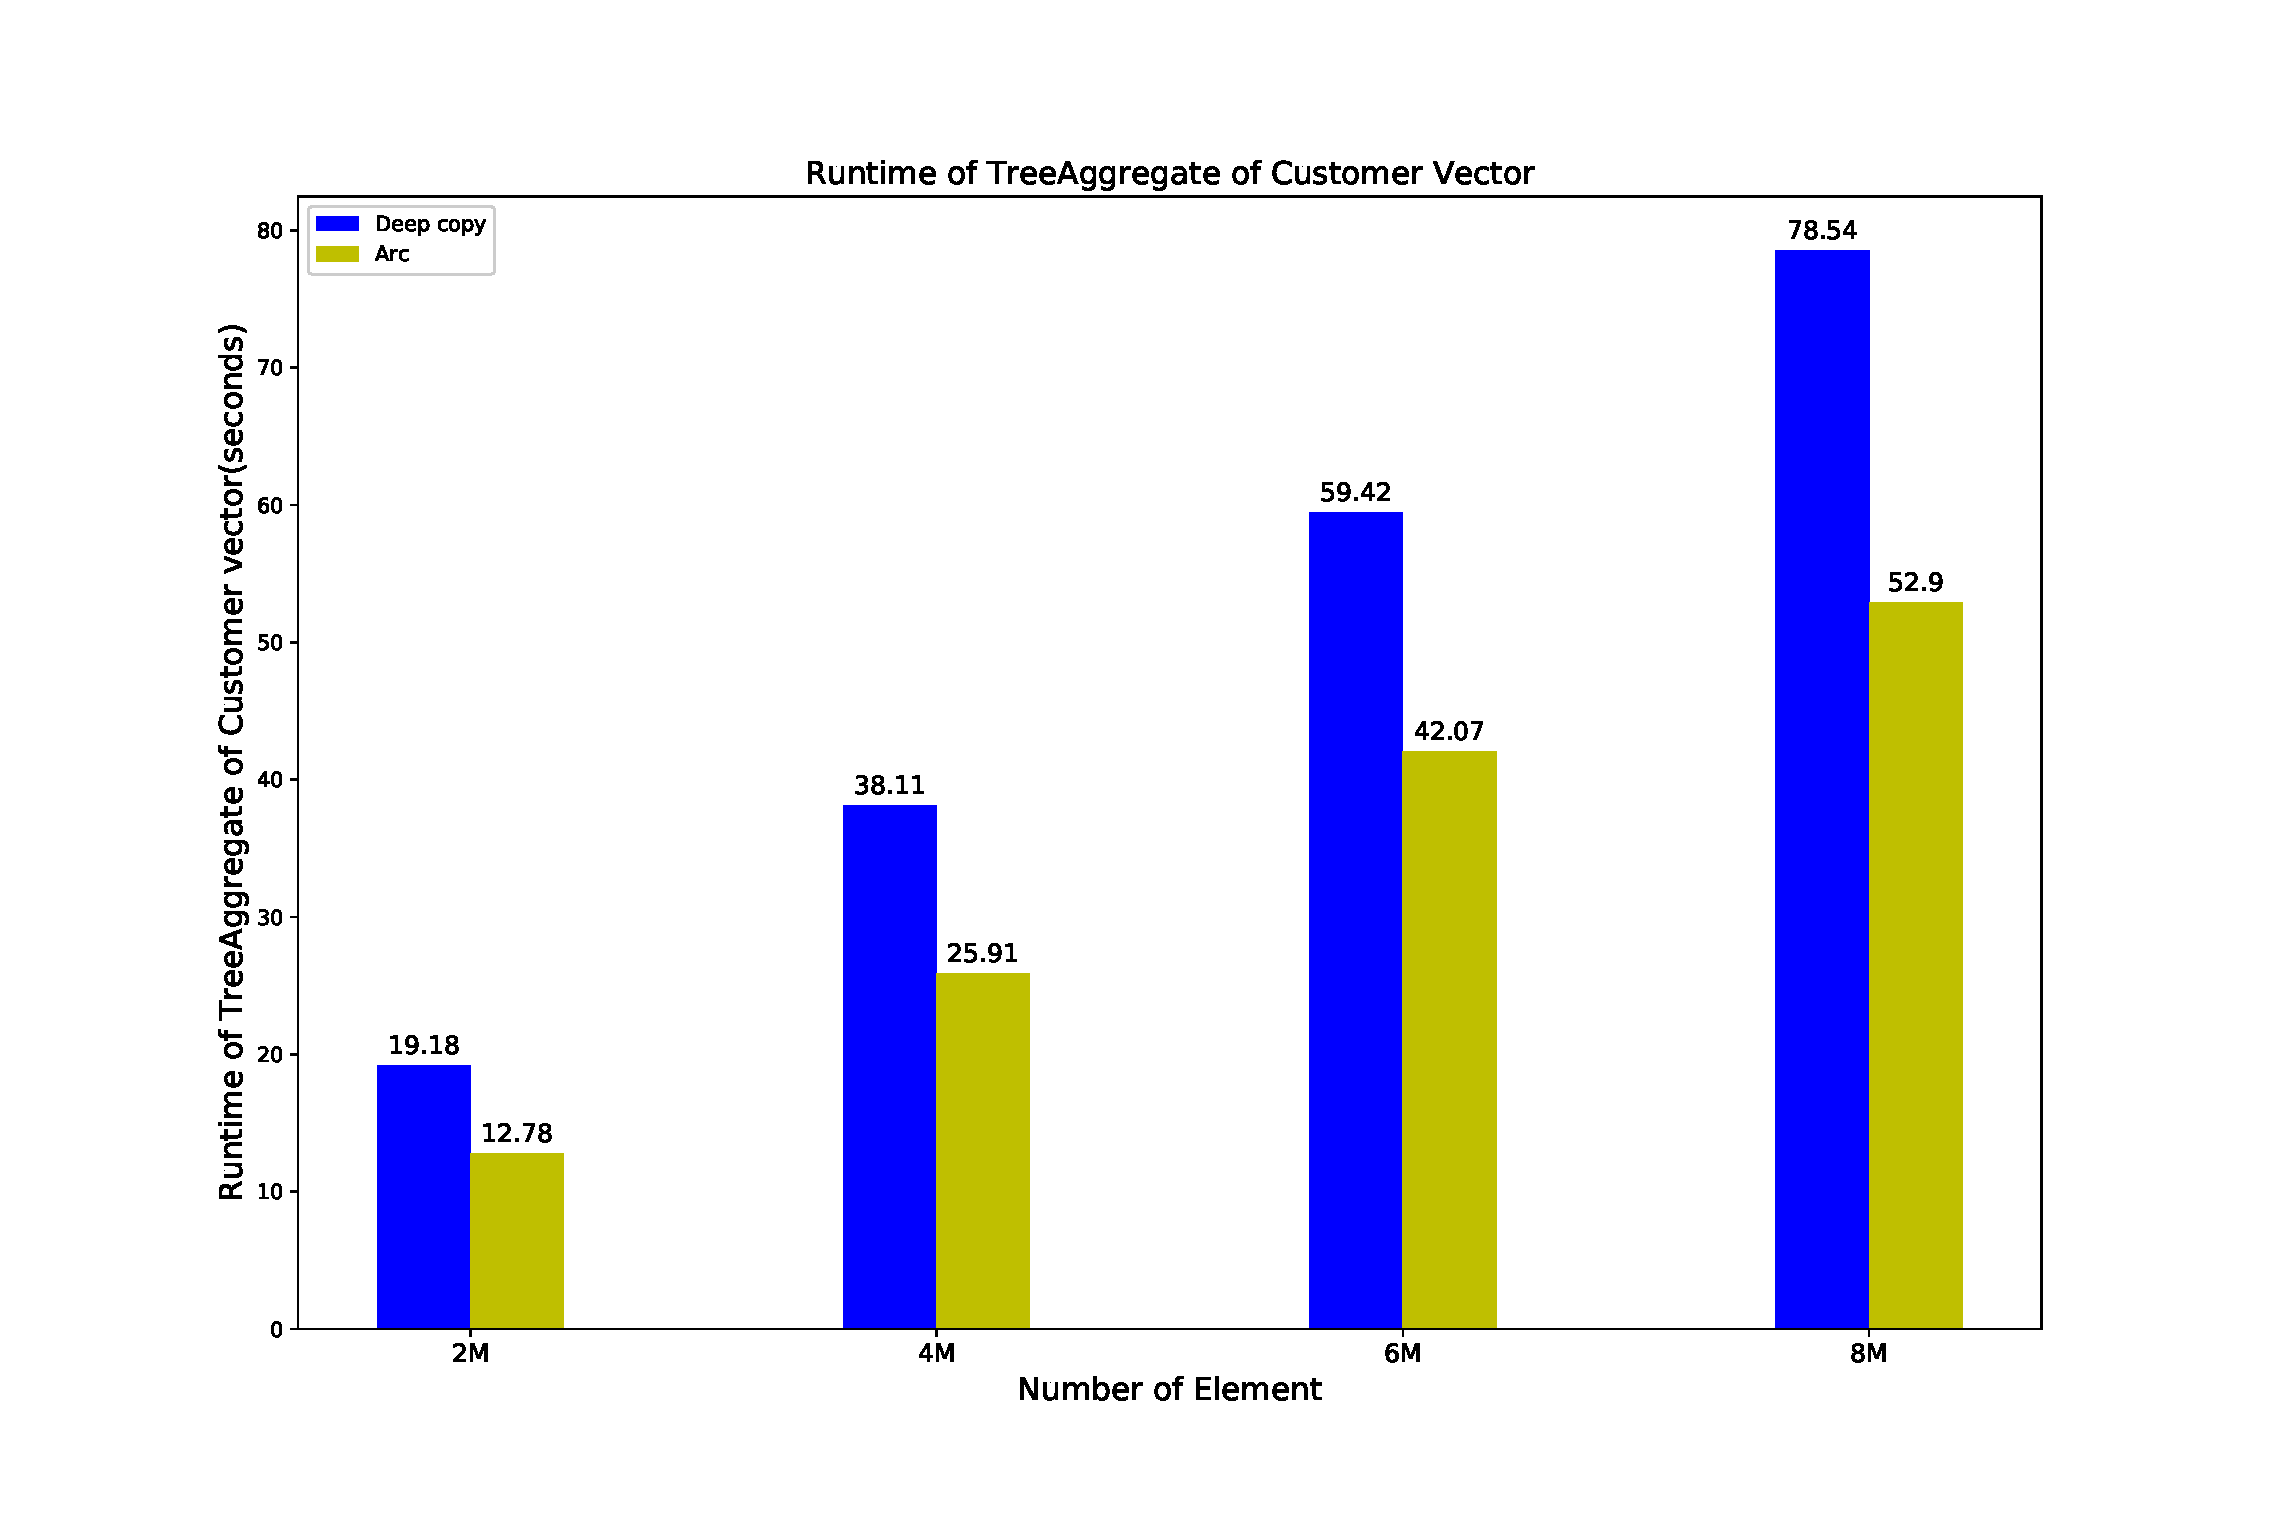
\includegraphics[width=15cm]{rust_tree_aggregate.eps}
    \caption{Runtime of Tree-aggregate algorithm}
    \label{fig:Sampling}
\end{figure}

\subsection{Discussion}
As we explained, Arc has overhead to be deleted because it has to check if the value is still referred. 
Even though the deletion of Arc is slow, deep copy of complex objects has more impact in deterioration of runtime performance. 
In the algorithm with deep copy, the elements of each partition in each node are deep-copied once during aggregation. 

If total number of elements are 1000000, the all of 1000000 elements are deep-copied once during execution. On the other hand, acquisition and deletion of Arc occurs several time for each element object.
First, acquisition of Arc of all elements in loaded vector happens during aggregation in each node and the loaded vector is deleted after the aggregation. 
Second, deletion of all elements in aggregated structures from children nodes and the node is occurs after joining these aggregated structures to single one. 

The result shows a deep-copy of Customer vector is computationally much more expensive than acquisition and deletion of Arc. 
This result suggests that having element objects in Arc is efficient than deep-copying element from original source vector in tree-aggregation algorithm 
where generates intermediate data structure. 

\section{Experiment 5: K-Nearest-Neighbors}
\label{sec:eval_knn}
Finally, we examine performance of a Machine Learning (ML) algorithms. 
The goal of this experiment is to evaluate better memory management strategies in ML algorithms developed with Rust.
We employ K-Nearest-Neighbors (KNN) for ML algorithm to be studied in our experiments.
Our KNN algorithms perform document classification on Wikipedia page data set described in Section~\ref{sec:eval_setdetail}. 

The algorithms have 4 phase; load, preprocess, query, and combine phase. 
Before these phase, we separate data sets into 8 partitions to run these in different threads. 
The algorithms spawn threads at the beginning ,and in the load phase partition of files are loaded in each threads. 
In preprocessing phase, the algorithm process document strings to generate Term-frequencies (Tfs) matrices and other data structures. 
In query phase, it calculates cosine similarities between all combination of train and test observations and select to top \(K\) nearest neighbors. 
In combine phase, the results from each batch and from each are combined. 
Based on our experiments result, the runtime in preprocess and query phase are significantly larger than other two phases.
Therefore, we focus discussion in these two phases considering them bottlenecks in our KNN algorithms.

KNN algorithms are implemented with different memory management strategies. 
We parametrize these memory management and some other values. These parameters are listed in Table~\ref{tab:parameter}. 

\begin{table}
    \renewcommand{\arraystretch}{1.2}
    \begin{tabular}{|l|l|l|l|l|}
    \hline
    Parameter Name  & \multicolumn{4}{l|}{Values and Description}                                                                                                                                                                                \\ \hline
    Method          & \multicolumn{4}{l|}{\begin{tabular}[c]{@{}l@{}}deep-copy:  use deep-copy to generate intermediate objects\\ arc: use atomic reference count to generate intermediate objects\end{tabular}}                                 \\ \hline
    Strategy        & \multicolumn{4}{l|}{\begin{tabular}[c]{@{}l@{}}1: keep intermediate objects in memory until owner is changed\\ 2: remove intermediate objects as soon as it is not needed\end{tabular}}                                    \\ \hline
    Number of batch & \multicolumn{4}{l|}{\begin{tabular}[c]{@{}l@{}}2: generate 2 batches from each partition\\ 3: generate 3 batches from each partition\end{tabular}}                                                                             \\ \hline
    k               & \multicolumn{4}{l|}{\begin{tabular}[c]{@{}l@{}}15K: dimension of feature matrices is 15 thousands \\ 20K: dimension of feature matrices is 20 thousands\\ 25K: dimension of feature matrices is 25 thousands\end{tabular}} \\ \hline
    \end{tabular}
    \caption{Parameter of KNN algorithms}
    \label{tab:parameter}
 \end{table}


Method parameter is specified to select memory management strategy used in preprocess phase. 
In preprocess phase, the algorithm generates many intermediate data structures using same String elements.
Deep-copy method deeply copies String to generate intermediate data structures. Arc method use Atomic Reference Count (Arc) to wrap String elements in the original data structure and 
clone Arc when the elements are used in other data structures. As Experiment 4 had shown in in Section~\ref{sec:eval_treeagg}, deep-copy of complex objects is more expensive than cloning Arc. 
String is a sort of objects allocated in heap and copied many times in preprocess phase. Therefore, it is worth to assess which method can be better memory management strategy in our experiments.

Strategy parameter controls memory management strategy used in both preprocess and query phase.
Strategy 1 keeps all intermediate data structures and numeric matrix objects from preprocess to query phase. 
Strategy 2 removes these data structures and objects as soon as they are not needed. 
These strategies differ from each other in terms of memory usage and frequency of memory deallocations.
These may cause significant runtime difference of the algorithms.

Number of batch controls number and size of batch for each partition. This parameter varies size of intermediate data structures and numeric matrices, and 
frequency of memory deallocations. 
The size of each batch is defined in 6250 pages when we have 2 batches, and 4166 or 4167 when we have 3 batches. 
The parameter k specifies number of dimension of feature matrices created out of preprocess phase. 
By controlling this, it determines size of intermediate data structures and numeric matrices. 

By controlling these parameter, we compare runtime and memory usage of KNN algorithms. 


\subsection{Result}
\label{sec:history}
Figure~\ref{fig:total}, ~\ref{fig:preprocess}, and ~\ref{fig:query} show the runtime performance of our KNN algorithms in total, preprocess, and query phase respectively. 
The algorithms used in our experiments are indexed in Table~\ref{tab:algorithm}. We call each algorithm in algorithm number for easy understanding.
The Algorithm 3 with 20K and 25K dimension, and the Algorithm 1 with 25K dimension whose runtime is showing 0 seconds are algorithms that are terminated during execution due to fail of memory allocation.

Figure~\ref{fig:total} shows Algorithm 8 shows much slower performance compare to the other algorithms.
Algorithm 7 also starts to slow down as we increase the number of dimension.  

As shown in Figure~\ref{fig:preprocess}, the algorithms using Arc is much slower than using deep-copy in preprocessing phase. 
Algorithm 8 is 38\%  slower than Algorithm 6 in dimension of 25K. 
In addition, the algorithms with strategy 2 are slower than with strategy 1. 
For example, Algorithm 6 is about 85\% slower than one Algorithm 2 in dimension of 25K.
The algorithms with 3 batches are slower that ones with 2 batches. Furthermore, as we increase the number of dimension, the number of batch becomes more and more critical to runtime performance of the algorithms with deep-copy.
The runtime ratios of difference from Algorithm 7 to Algorithm 8 are about 44\%, 28\%, and 39\% for dimension of 15K, 20K, and 25K respectively. 
However, those from Algorithm 5 to Algorithm 6 are about 11\%, 28\%, and 54\%. The ratios of difference increase proportionally to the number of dimension. 

In query phase, Algorithm 8 is much slower than the others in different parameter settings.
Algorithm 7 starts to slow down as number of dimension is increased. 


\begin{table}
    \renewcommand{\arraystretch}{1.2}
    \begin{tabular}{|l|l|l|l|}
    \hline
    Algorithm number & Method    & Strategy & Number of batch \\ \hline
    1                & deep-copy & 1        & 2               \\ \hline
    2                & deep-copy & 1        & 3               \\ \hline
    3                & arc       & 1        & 2               \\ \hline
    4                & arc       & 1        & 3               \\ \hline
    5                & deep-copy & 2        & 2               \\ \hline
    6                & deep-copy & 2        & 3               \\ \hline
    7                & arc       & 2        & 2               \\ \hline
    8                & arc       & 2        & 3               \\ \hline
    \end{tabular}
    \caption{Index of Algorithm}
    \label{tab:algorithm}
 \end{table}

\begin{figure}[htb]
    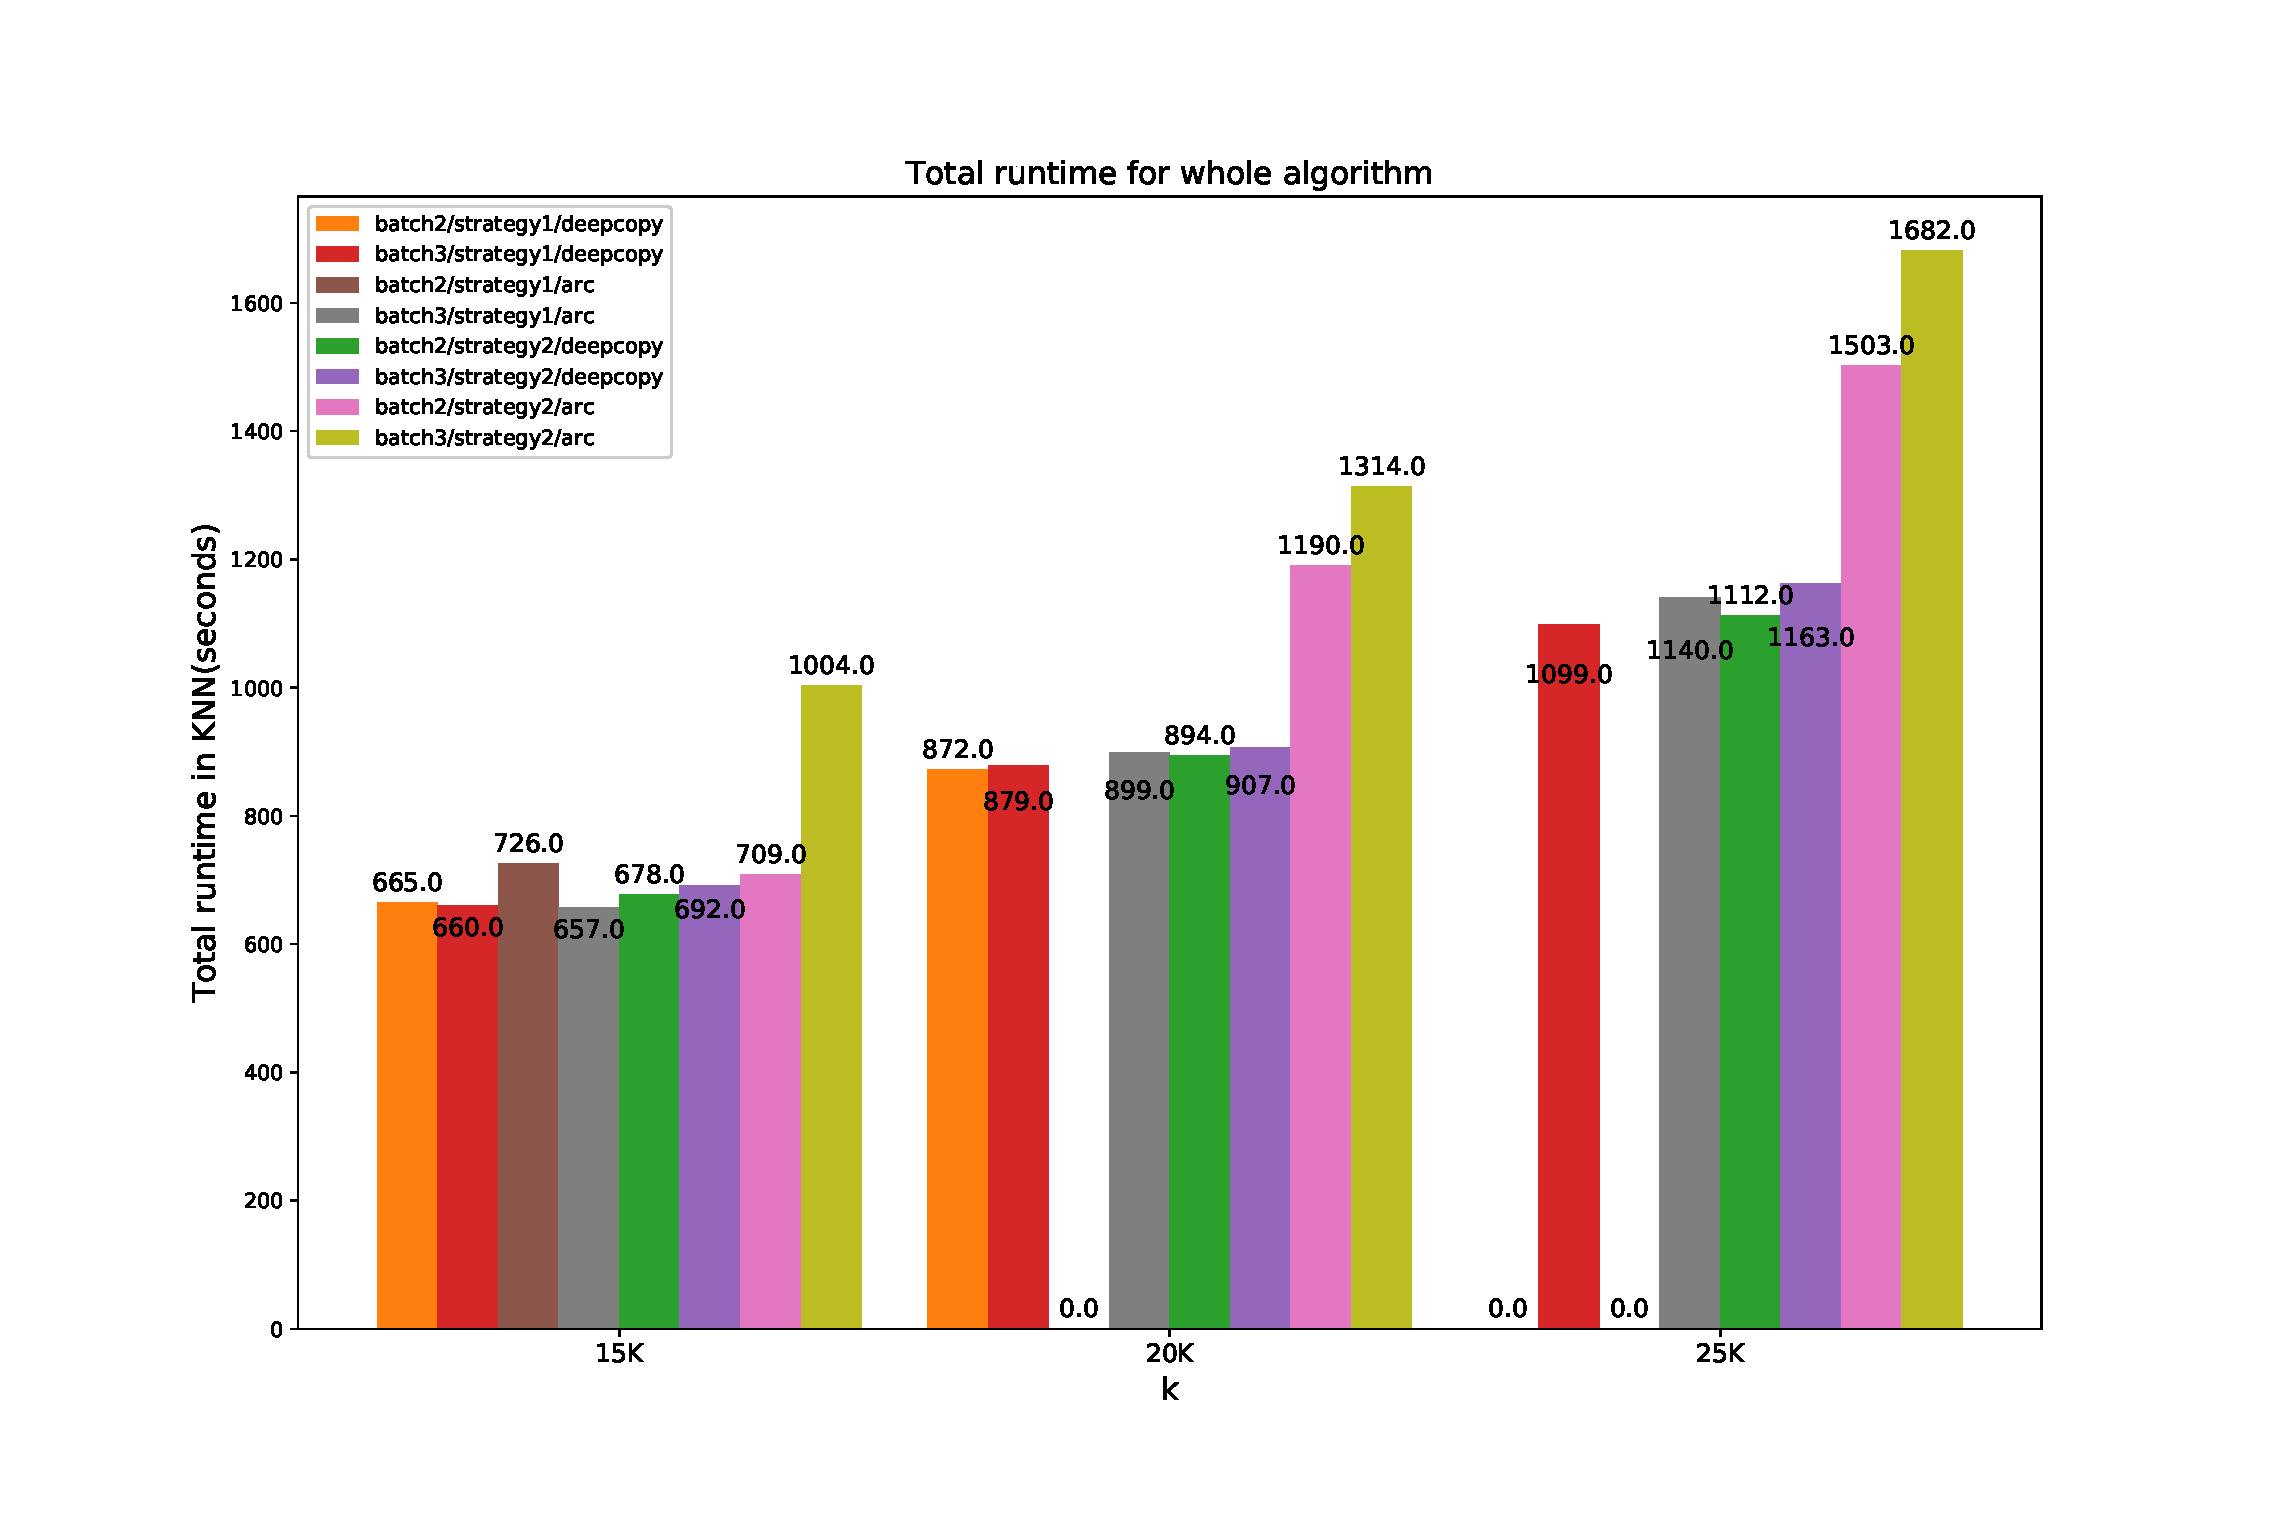
\includegraphics[width=15cm]{total.eps}
    \caption{Total runtime whole KNN algorithm (seconds)}
    \label{fig:total}
\end{figure}

\begin{figure}[htb]
    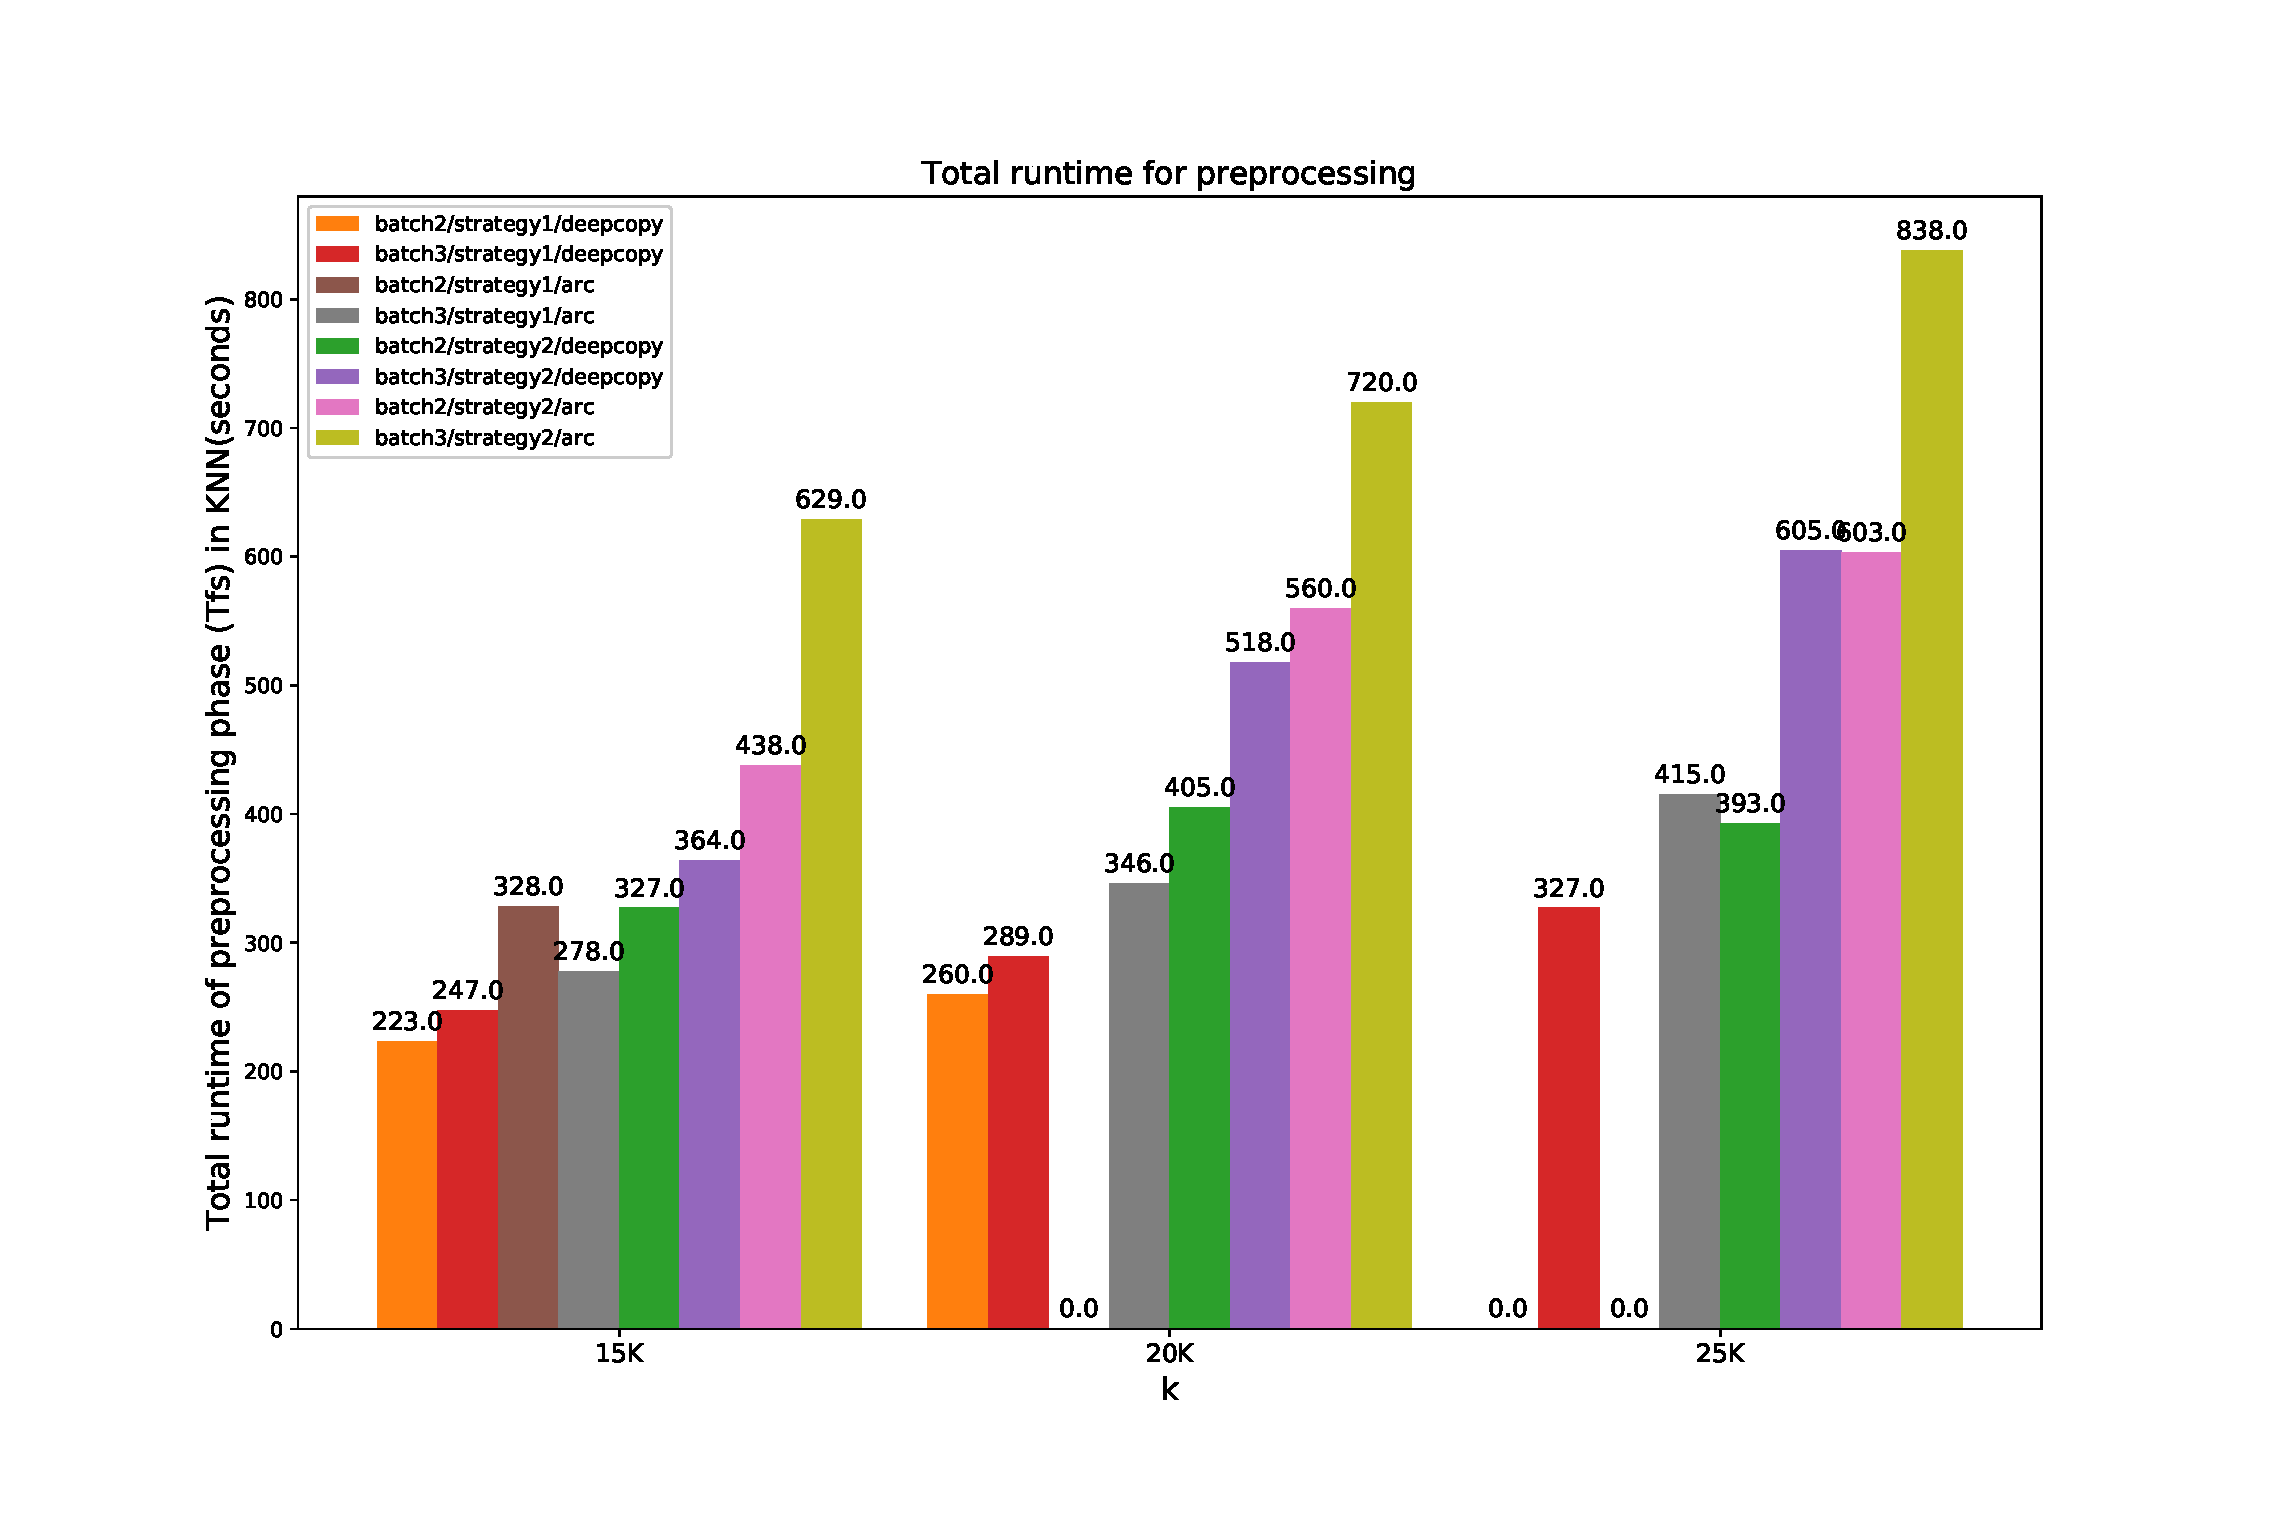
\includegraphics[width=15cm]{preprocessing.eps}
    \caption{Total runtime of preprocessing phase in KNN (seconds)}
    \label{fig:preprocess}
\end{figure}


\begin{figure}[htb]
    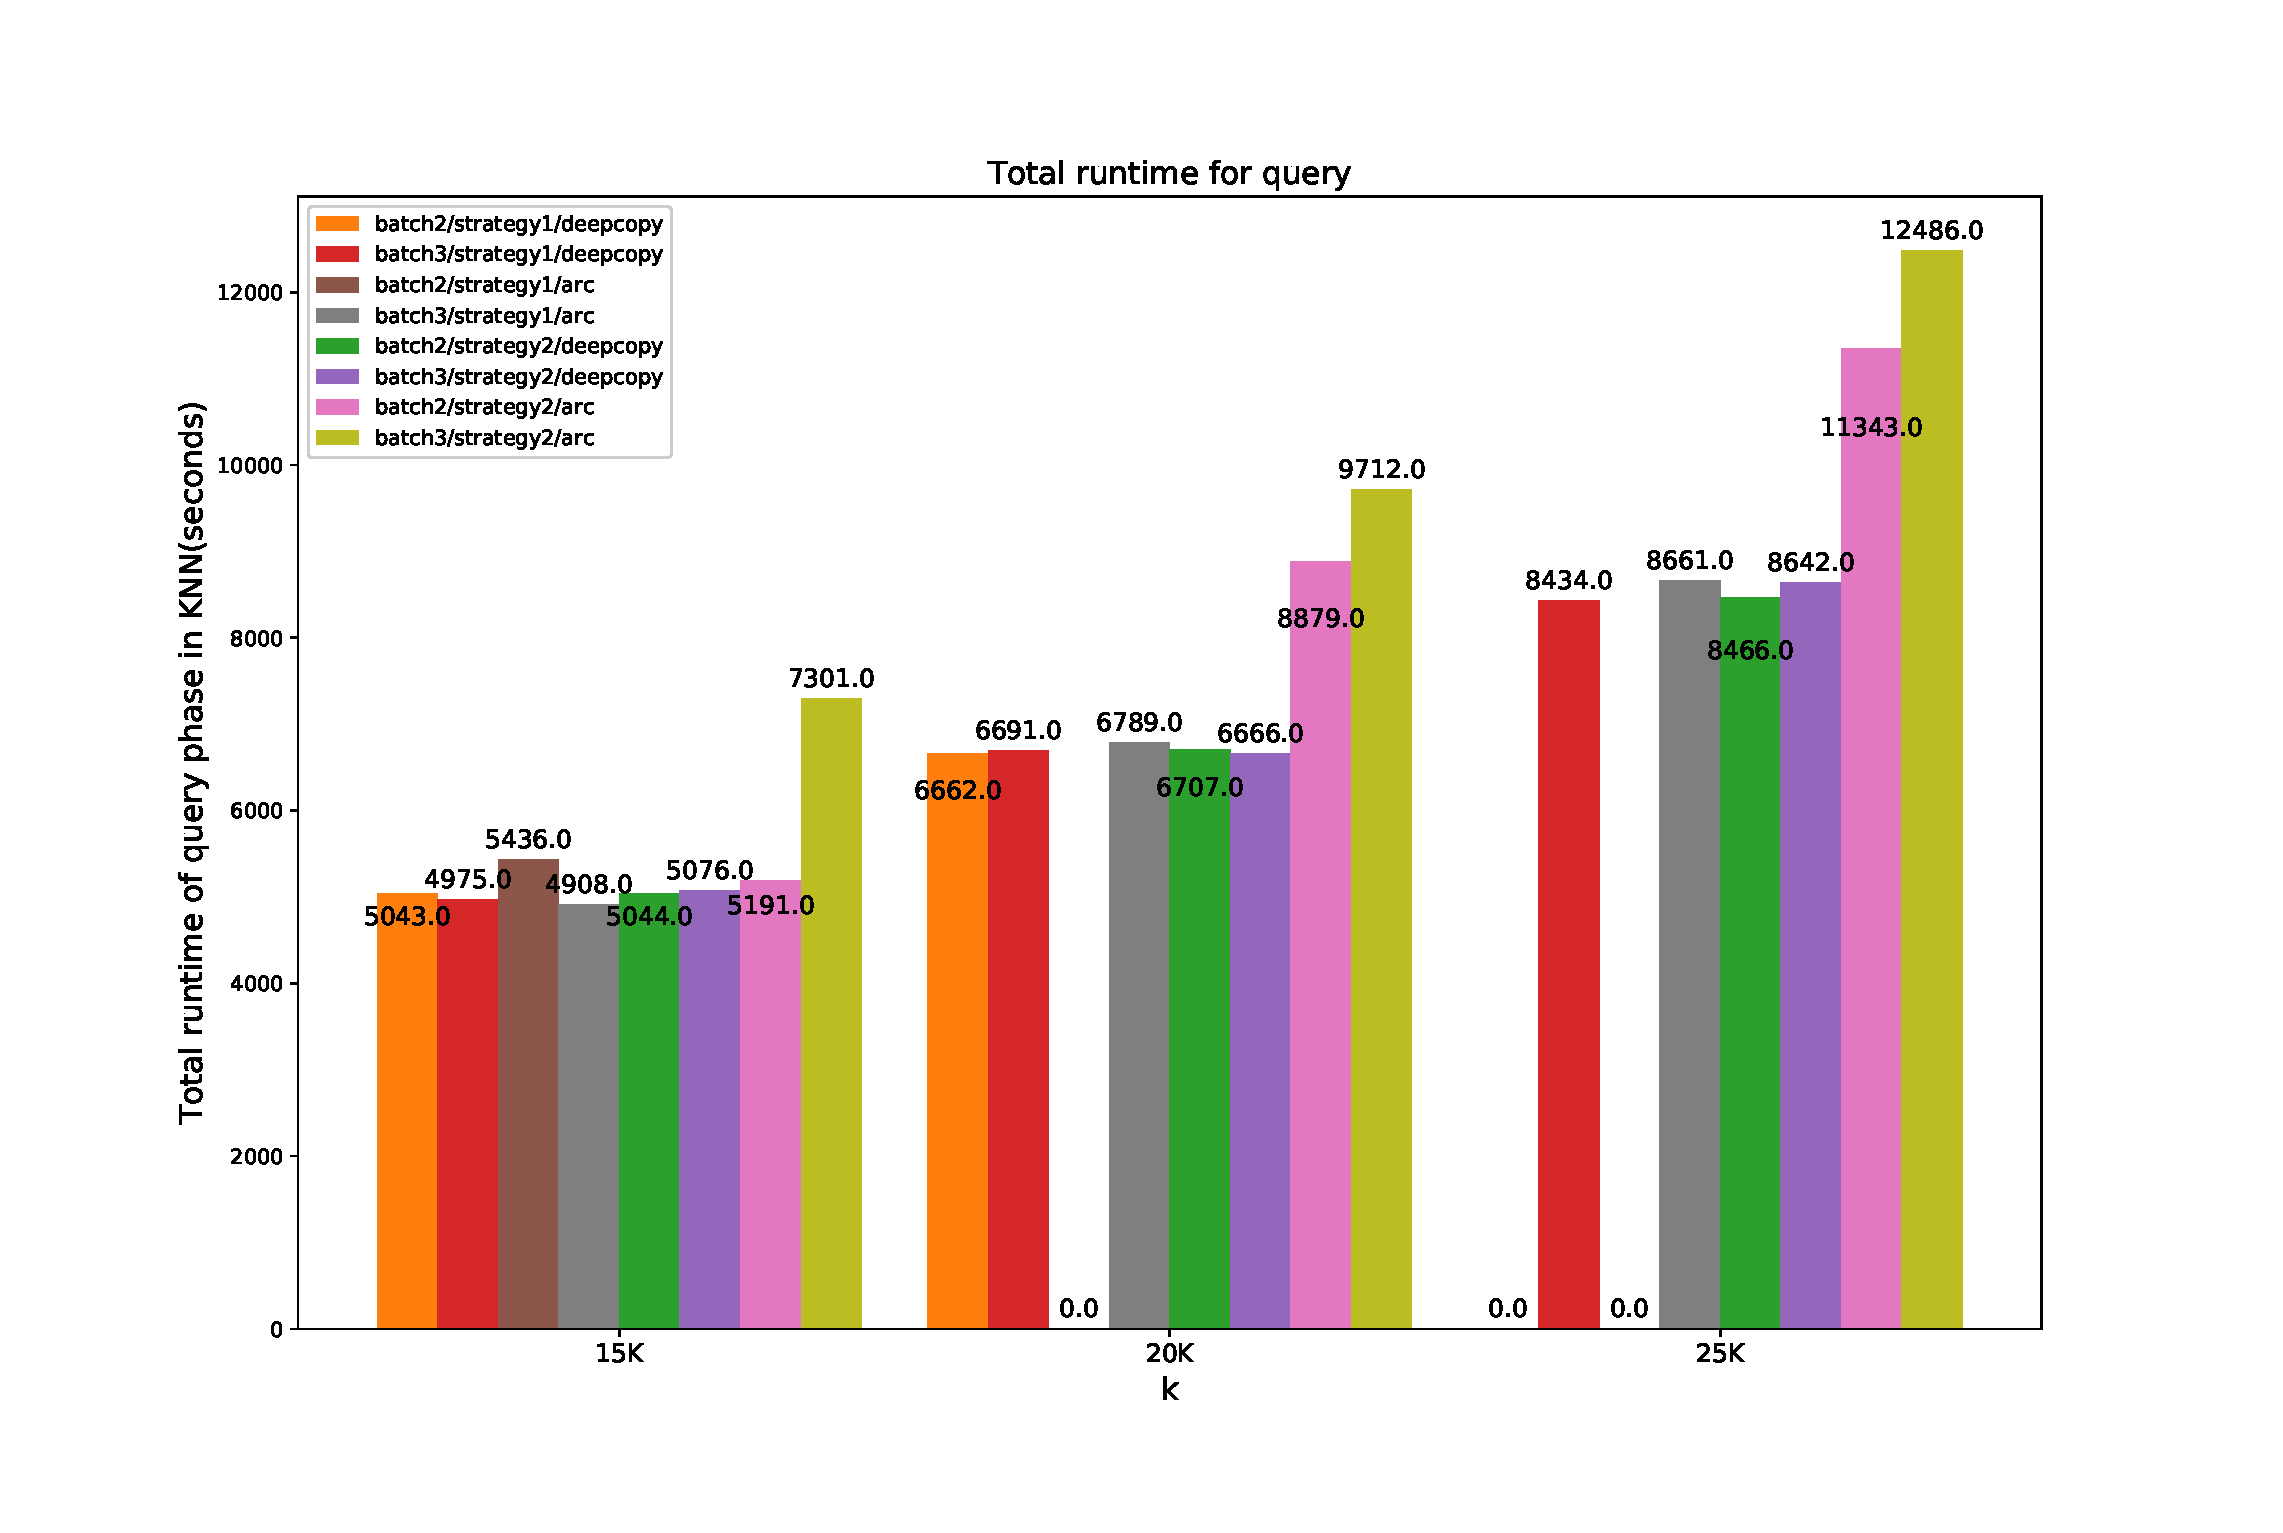
\includegraphics[width=15cm]{query.eps}
    \caption{Total runtime of query phase in KNN (seconds)}
    \label{fig:query}
\end{figure}


\subsection{Discussion}
\label{sec:history}
In preprocess phase, the algorithms using Arc method performs worse than ones with deep-copy method. 
This result may seem to contradict to the result of Experiment 4 in Section~\ref{sec:eval_treeagg}.
In Experiment 4, complex objects, CustomerOwned, are cloned with Arc or deep-copied. 
In this Experiment 5, we however get Arc or deep-copy of String instead of complex object.
The result explains deep-copying String is much inexpensive than deep-copying the complex object and 
using deep-copy method is actually efficient than using Arc to share String. 
Therefore, we need to make decision which method to use depending on size and complexity of objects.

In addition, use of different strategies in preprocess phase explains how deallocations of intermediate data structures and drops of their variables impact algorithm's runtime performance.
The result shows deallocations of intermediate data costs a lot; Algorithm 6 is 85\% slower than Algorithm 2.
This may be more severe bottleneck for algorithms using Arc; Algorithm 8 is 102\% slower than Algorithm 4.
This is the same reason explained in Experiment 4. 
Arc has to check reference count and its atomic operation is expensive. 

The impact of batch number can explain how frequency of memory de/allocation affects runtime performance. 
Dealing with more number of batch has negative impacts on runtime performance because it triggers more frequent memory de/allocation.
In addition, as we increase the number of dimension, the ration of runtime difference among different numbers of batch for the algorithms with deep-copy, but not for ones with Arc.
This is because algorithm with Arc does not de/allocate memory as much frequent as ones with deep-copy.
The intermediate data structures mealy get reference to String values without actually allocating memory for copied Strings.

In query phase, most of our algorithms shows similar runtime performance among the same number of dimension. 
Why such differences seen in preprocess phase are not shown in query phase? This is because the data structures processed in this phase are numeric matrices and vectors. 
These data structures do not contain String so that the selection of method parameter does not have direct impact to algorithm's runtime performance.

Furthermore, numeric matrices and vectors are contiguously allocated initializing their size, so they are easy to be de/allocated. 
The computation needed for these de/allocations is fairly fast. Therefore, setting parameters, such as number of batch and strategy, does not impacts runtime performance.

However, we can see significant degradation in Algorithm 7 with 20K and 25K dimension and Algorithm 8 with 15K, 20K, and 25K dimension. 
By using strategy 2, we deallocate the numeric matrices and vectors in query phase. However, it is difficult to think that these contiguous memory deallocations cause the degradation. 
If that is so, Algorithm 5 and 6 should also show some overheads. No page-swapping does not happen during the execution. 
One possible reason is that these algorithms suffer from the allocation of numeric matrices and vectors due to previous deallocation of intermediate data structures in preprocess phase. 
The frequent deallocations and low locality of Arc may lead long free-space-list making difficult to search enough spaces to allocate numeric matrices and vectors.
The other possibility is that the frequent deallocations and low locality of Arc cause cache of numeric matrices and vectors. 
The computation on these numeric objects may slow down due to their caching levels. 
To conclude these discussion, we need to conduct more experiments and deeper analysis. 
However, we push those discussion in next paper.

In a part of conclusion, using Arc to String may be overhead. Considered the result from Experiment 4, we need careful consideration which object to use which strategy, deep-copy and Arc.
In addition, frequent memory deallocation can lead to slower runtime performance. 
Therefore, we need to decide when to deallocate unused values taking account of memory capacity. 


\section{Summary}
\label{sec:eval_summary}

% \section{Elements Copy and Insertion into Size-initialized Vector in Rust.}
% \label{sec:history}
% In this experiment, four methods are used to insert elements into vector in Rust. One is clone method which performs bitwise deep copy. 
Another is clone\_from which also performs bitwise deep copy, but copies elements of the vector to distination vector rather than 
creating new one. We initialize the distination vector with the same size to the number of elements we insert into it. 
Another is copy\_nonoverlapping function which copies values from source to distination memory region. 
The other is pushing elements of source to distination vector one by one. Insertions of elements with 4 size are conducted 1000000, 1500000, 10000000, 15000000, and, 
their runtimes for each elements type, integer and String are measured. 


The figure shows the result of the experiment. Among the runtime performances of integer insertion for every methods, 
clone, clone\_from, and copy\_nonoverlapping method shows the similar performance. However, the pushing the copy of elements one by one has much slower runtime performance 
compared to the rest. This is because integer elements are allocated contiguously in the memory, so that accessing address of memory by pointer reads some next address. 
This boosts the copy and insertion of elements. 

On the other hand, all of methods show the similar runtime performance in experiment for String object insertion. 
This is because String object is not stored in contiguous memory region. The vector stores pointer to the object and 
process need to access around different memory region again and again to deeply copy the object.

\begin{figure}[htb]
    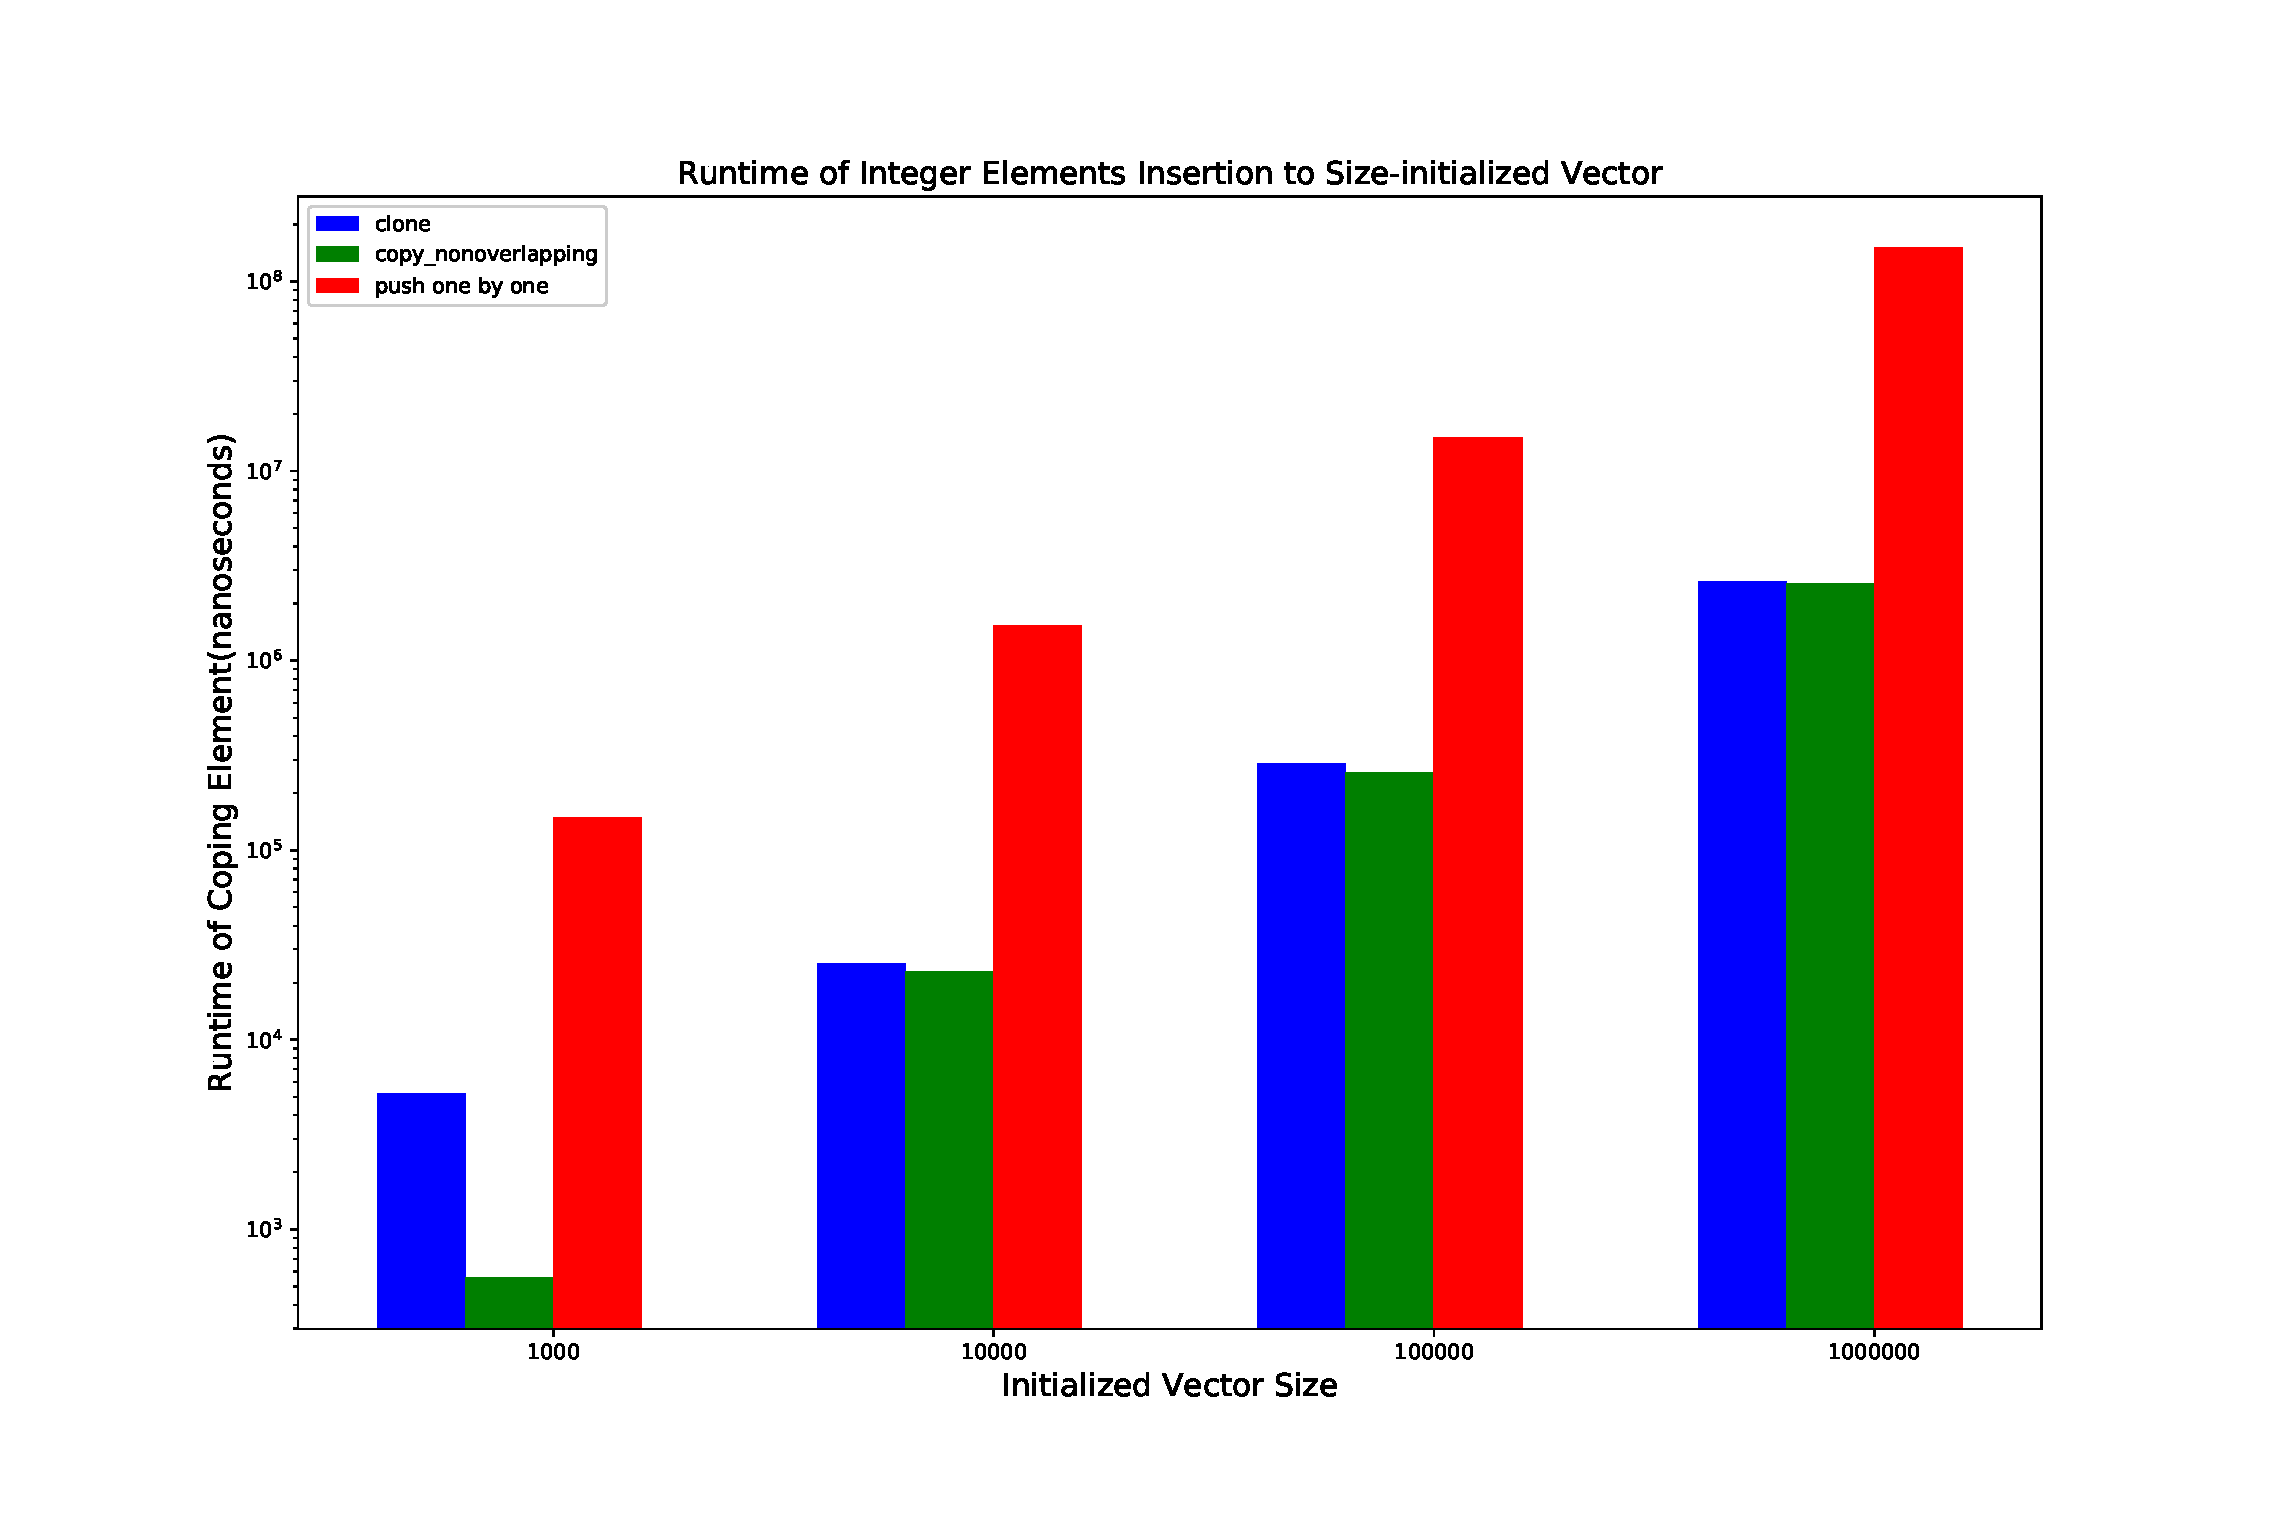
\includegraphics[width=15cm]{rust_various_insertion.eps}
    \caption{Runtime of elements copy from one vector and insertion to the other vector.}
    \label{fig:Sampling}
\end{figure}
\clearpage

\section{Access time to elements in vector}
\label{sec:history}
In this experiment, whether mutability has impacts to operation on the object in terms of runtime performance. 
According to the experiment, there is no difference on accessing to elements of mutable and immutable vector.

\begin{figure}[htb]
    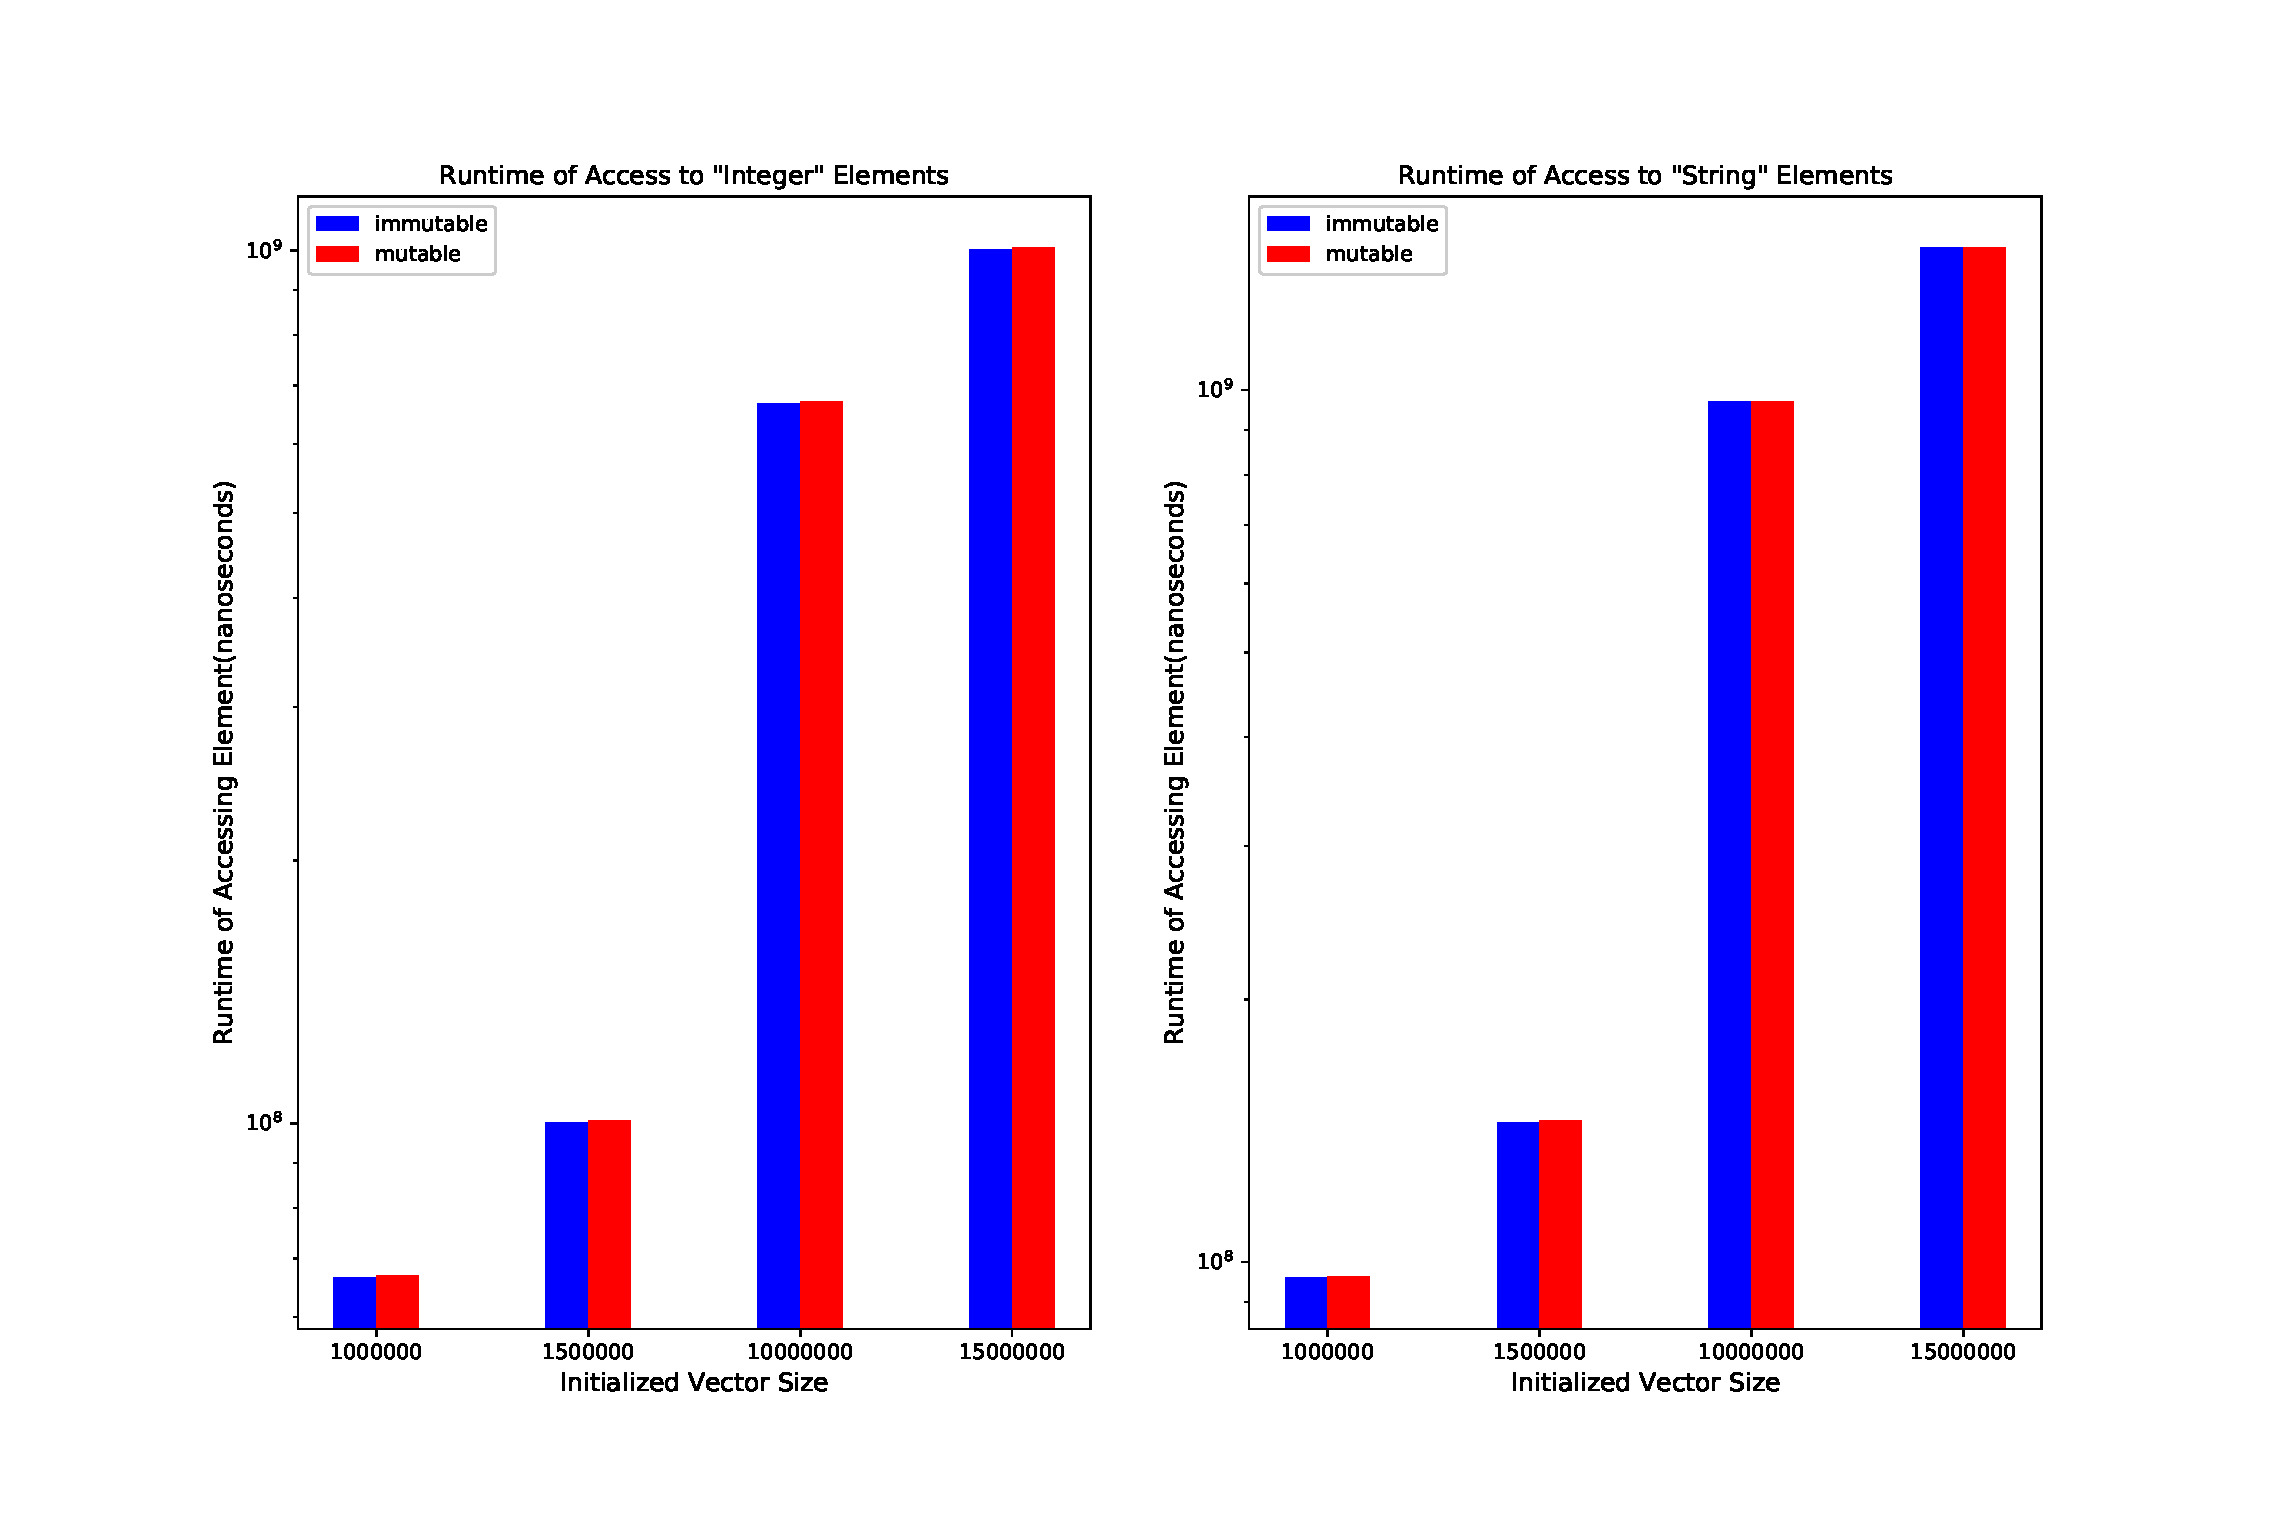
\includegraphics[width=15cm]{rust_various_access.eps}
    \caption{Runtime of elements copy from one vector and insertion to the other vector.}
    \label{fig:Sampling}
\end{figure}



